 \documentclass[12pt,titlepage]{article}


\usepackage{nomencl}
\usepackage[american]{babel}
\usepackage[utf8]{inputenc}
\usepackage[T1]{fontenc}
\usepackage{lmodern}
\usepackage{amsmath,amsfonts,amssymb}
\usepackage{graphicx}
\usepackage{geometry}
\geometry{a4paper}
\usepackage[parfill]{parskip}
\usepackage{graphicx}
\usepackage{amssymb}
\usepackage{epstopdf}
\usepackage{color}
\usepackage[tt]{titlepic}
\usepackage{fancyhdr}
\usepackage{enumerate}
\usepackage{lastpage}
\usepackage{bm}

\usepackage{listings}
\definecolor{codegreen}{rgb}{0,0.6,0}
\definecolor{codegray}{rgb}{0.5,0.5,0.5}
\definecolor{codepurple}{rgb}{0.58,0,0.82}
\definecolor{backcolour}{rgb}{0.95,0.95,0.92}
 
\lstdefinestyle{mystyle}{
	language=Python,
    backgroundcolor=\color{backcolour},   
    commentstyle=\color{codegreen},
    keywordstyle=\color{blue},
    numberstyle=\tiny\color{codegray},
    stringstyle=\color{codepurple},
    basicstyle=\footnotesize,
    breakatwhitespace=false,         
    breaklines=true,                 
    captionpos=b,                    
    keepspaces=true,                 
    numbers=left,                    
    numbersep=5pt,                  
    showspaces=false,                
    showstringspaces=false,
    showtabs=false,                  
    tabsize=2,
    deletekeywords={filter, map, open, complex}
}

\lstset{style=mystyle}
\usepackage[section]{placeins}
\usepackage{amsfonts}
\usepackage{amsmath}
\usepackage{float}
\usepackage{setspace}
\usepackage[justification=centering]{caption}
\usepackage{sidecap}
\usepackage{subcaption}
\usepackage{multirow}
\usepackage[squaren, Gray, cdot]{SIunits}
\graphicspath{{image/}} %chemin par défaut pour aller chercher les images 
\usepackage{url}

% FOR DEFINITIONS (https://www.sharelatex.com/learn/Theorems_and_proofs)
\usepackage{amsthm}
\theoremstyle{definition}
\newtheorem{definition}{Definition}[section]
\newtheorem*{definition*}{Definition}
\newtheorem{prop}{Proposition}
\newtheorem*{prop*}{Proposition}
\theoremstyle{remark}
\newtheorem*{remark}{Remark}
\newtheorem*{corollary}{Corollary}
\newtheorem{theorem}{Theorem}[section]
\newtheorem{lemma}[theorem]{Lemma}
\newtheorem*{example}{Example}

% Custom Defines
\usepackage[comma,numbers,sort&compress]{natbib}
\bibliographystyle{plainnat}
\usepackage[pdfstartview=FitH,
            breaklinks=true,
            bookmarksopen=true,
            bookmarksnumbered=true,
            colorlinks=true,
            linkcolor=black,
            citecolor=black
            ]{hyperref}
\newcommand{\rmd}{\textrm{d}}
\newcommand{\bi}[1]{{\ensuremath{\boldsymbol{#1}}}}
\definecolor{gray}{rgb}{0.5,0.5,0.5}

\topmargin=-0.45in      %
%\evensidemargin=0in     %
\oddsidemargin=-0.1in      %
\textwidth=6.8in        %
\textheight=9.2in       %
%\headsep=0.25in         %
\headheight=30.9pt

\begin{document}

% ========== TITLE PAGE ===================================================

\begin{titlepage}
\newcommand{\HRule}{\rule{\linewidth}{1mm}} % Defines a new command for the horizontal lines, change thickness here

\center % Center everything on the page

\includegraphics[width=8cm]{images/polimi.png}\\[1.5cm]

%	HEADING SECTIONS
\textsc{\LARGE Advanced Programming for \\[0.1cm]Scientific Computing}\\[1.cm]

%	TITLE SECTION
\HRule \\[0.4cm]
{ \huge \bfseries A Python/C++ package for \\[0.4cm] Predictive Topological Data Analysis}\\[0.4cm] 
\HRule \\[1.5cm]     

%	AUTHOR SECTION
\begin{minipage}{0.4\textwidth}
\begin{flushleft} \large
\emph{}\\
Martino \textsc{Milani}\\
\end{flushleft}
\end{minipage}
~
%	DATE SECTION
{\large \today }\\[2cm] % Date, change the \today to a set date if you want to be precise
\vfill % Fill the rest of the page with whitespace
\end{titlepage}
%\onehalfspacing

% ========== HEADER =======================================================
\pagestyle{headings} \pagenumbering{arabic} \setcounter{page}{1}
\addtolength{\headheight}{\baselineskip}
\lhead{\textbf{Martino Milani}}
\chead{PACS}
\renewcommand{\headrulewidth}{0.4pt}


\begin{abstract}

A fundamental problem in data analysis is the visualization of high dimensional datasets. \\G. Carlsson et al. in \cite{topologyanddata} propose an algorithm called Mapper that visualizes the dataset through a simplicial complex that aims at approximating the topology of the dataset. Few implementations of this algorithm already exist \cite{KMapper, pythonmapper}; in this work we propose lmapper, a Python package that provides an alternative, efficient and easily extensible implementation of Mapper. We benchmarked lmapper against \cite{KMapper} on two different datasets and verified that in both cases lmapper is faster and more robust to noise. We then present a companion Python package, filterutils, written in C++ with the use of OpenMP for higher performances.\\
Palma et al. in \cite{Palma} proposed a binary classification algorithm based on Mapper; in this work we developed on top of lmapper a third package, predmap, implementing such algorithm. With predmap we were able in a simple case (majority vote) to retrieve the same results presented in \cite{Palma}.

\end{abstract}
\pagebreak

\tableofcontents
\pagebreak

%\listoffigures
%\listoftables
%\pagebreak


%*******************************************************************************
%*********************************** First Chapter *****************************
%*******************************************************************************


\setcounter{page}{1}
\ifpdf
\graphicspath{{Figs/}}
\else
\graphicspath{{Figs/}}
\fi


%********************************** %First Section  **************************************
\section {Topological Data Analysis and Mapper} 

\paragraph{}
One way for scientists to make sense of complex data is to identify groups (clusters) of similar data points. Instead of thinking of each data point as an individual entity we wish to identify a small number of meaningful groups and being able to label them makes scientists able to describe datasets with only a little information; the data point is seen as part of a bigger entity: the cluster which it belongs to. By neglecting differences between data points belonging to the same cluster, it is possible to achieve a very effective and compressed description of the dataset. Many clustering algorithms have been developed so far; most common algorithms, such as Gaussian Mixture Models, are founded on a probabilistic model that is build on the data. Other algorithms include optimization methods (k-means for example), density-based methods and hierarchical algorithms \cite{handbook_of_cluster}.

\begin{figure}[htbp!] 
	\centering    
	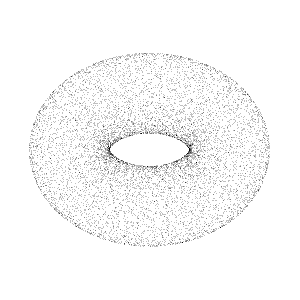
\includegraphics[width=0.2\textwidth]{Point_cloud_torus.png}
	\caption{A data point cloud sampled from a torus in $\mathbb{R}^3$}
	\label{fig:torus}
\end{figure}

In the work of G. Carlsson et al. \cite{extracting_insights} a new algorithm called Mapper, based on a different approach, was presented. The observed points are thought not as sampled from a distribution, such as in GMM, but are thought to be sampled form an ideal object $\mathcal{O}$ with a particular shape; Mapper tries to visualize this shape. The concept of shape of a high-dimensional object is although non trivial, but tools to study the shape of such high-dimensional objects were already available in literature before Mapper: Reeb graphs. Reeb graphs manage to describe in a compact way information about an object $\mathcal{O}$ by keeping track of the evolution of the topology of the connected components of the level sets $f^{-1}(c), c\in \mathbb{R}$ of a function $f:\mathcal{O}\rightarrow\mathbb{R}$\cite{reebgraphs} \cite{biasotti}. The object $\mathcal{O}$ is however only an abstraction; inspired from the Reeb graphs, Mapper is an algorithm that implements this same idea but on the finite collection of data points, where the notion of "connected component" and level set are not well defined as on the ideal object $\mathcal{O}$. The output of Mapper can be thought of  as the skeleton of the shape of the object $\mathcal{O}$ from which the points are imagined to be sampled.  Thanks to a careful visual analysis of this skeleton we can improve our understanding of the dataset, and thus it is sometimes possible to perform a finer and more meaningful clustering of the datasets than with traditional algorithms \cite{extracting_insights}. In the following paragraph a first example of an application of Mapper is presented, in order to introduce the reader to the algorithm. With this example we want to provide the reader just with a first intuition of Mapper and introduce him to concepts such as filter function and distance; in the next section a formal definition of Mapper is provided.

\paragraph{A first example} 
In this first introductory example, taken from \cite{extracting_insights}, a three dimensional dataset is analyzed, since it is possible to visualize the data point cloud and get an understanding of the "shape" of the dataset just by looking at it.\newline 
The set of data points $X$ is represented in figure \ref{fig:hand}. A shape of a hand is recognizable. First, we need to define a distance $d$ on the data point cloud, in order to be able to introduce a notion of "closeness" between points, onto which a notion of connectedness of the data point cloud is based. In this way Mapper will be able to recognize points belonging to the same finger as part of the same connected component. A connected component of the object $\mathcal O$ is subset of $\mathcal O$ that cannot be represented by the union of two other disjoint subsets. \\
For the next definition the concept of metric space is needed. The readers not familiar with metric spaces can think for now about a metric space as a finite collection of points $X$ equipped with a function $d$ that associates to each couple of points $x,y\in X$ a scalar value that represent a measure of how far these two points are. For a formal definition of metric space, see definition \ref{def:metric}. 
\begin{definition}{[\textit{data point cloud}]}
	A \textbf{data point cloud} is a \textit{finite} metric space $(X,d)$ where $X \subset \mathbb{R}^n$ and $d$ is some distance in $\mathbb{R}^n$. 
\end{definition}

For this example, the euclidean distance $d(x,y)=\sqrt{(x_1-y_1)^2+(x_2-y_2)^2+(x_3-y_3)^2}$ is chosen. After this step, Mapper requires to define a function $f$ on the data point cloud $(X,d)$, called a \textit{filter function}. 
\begin{definition}{[\textit{filter function}]}
	A \textbf{filter function} is a continuous function $f \colon (X,d)\rightarrow \mathbb R$. 
\end{definition}
The chosen filter function $f : (X,d) \rightarrow \mathbb{R}$ is the $x$-coordinate of the points in $X$. In figure \ref{fig:hand} B) the points are colored by the value of the filter function, where blue means low values and red high values. The image $f(X)\subset \mathbb{R}$ is then binned into six, equally spaced, overlapping intervals $\{B_i\subset \mathbb R \colon \bigcup_{i=1}^6B_i = f(X)\}$. The data point cloud $(X,d)$ is then subdivided into six corresponding subsets $\{A_i\subset X \colon A_i = f^{-1 }(B_i)\}_{i=1}^6$ represented in figure \ref{fig:hand} C. Notice that, since the intervals $B_i$ were overlapping, the subsets $A_i=f^{-1}(B_i)$ in figure \ref{fig:hand} C share some points between them. On each of the six subsets $A_i$ , a clustering algorithm that makes use of the distance $d$ defined on $X$ is run. The clusters obtained represent in some way the notion of connected components of each $A_i\subset X$: if two points were close enough to be clustered together, they belonged to the same connected component. One node for each connected component obtained so far is created (figure \ref{fig:hand} D ). An edge is drawn only between the nodes representing connected components that share at least one point.

\begin{figure}[htbp!] 
	\centering    
	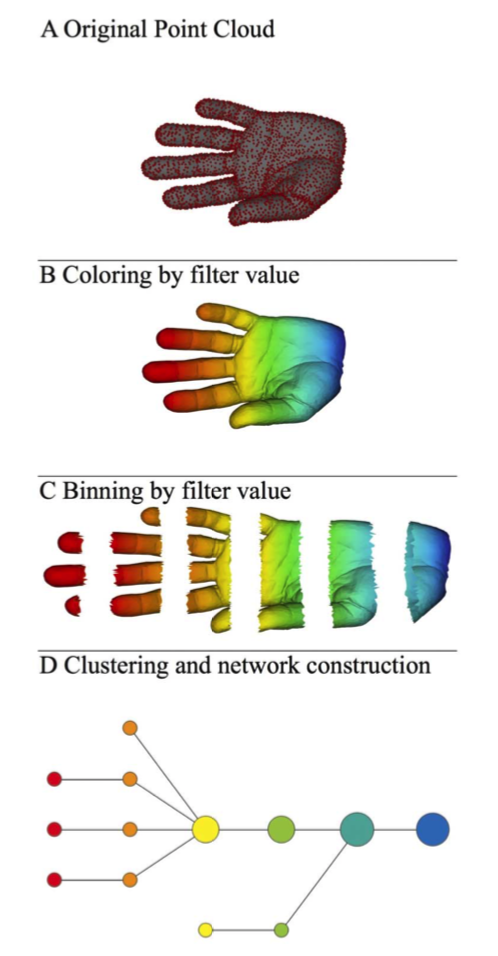
\includegraphics[width=0.3\textwidth]{mapper_first_example}
	\caption{A data point cloud with the shape of a hand; A) the data point cloud $X$ B) $X$ is colored by the values of the filter function $f$  C) $X$ is split into six subsets $\{A_i\}_{i=1}^6$ D) each connected component of each subset $A_i$ is represented by a node in the graph. An edge is drawn between the nodes corresponding to connected components that share at least one point. \textit{Figure from G. Carlsson et al, \cite{extracting_insights}}}
	\label{fig:hand}
\end{figure}

In the next section we adopt a rigorous approach to define Mapper. If the reader needs further examples, we suggest reading the paper of G. Carlsson \textit{et al.} \cite{extracting_insights} where the authors provide an introduction to Topological Data Analysis and Mapper and give three examples of applications of Mapper to represents the shape of datasets representing player performance data from the NBA, voting data of the House of the Representatives and gene expression data from breast tumors. 

%********************************** %Second Section  *************************************
\subsection{Introduction to topology}
%Section - 1.3
Many of the following definitions, notations and theorems, although sometimes slightly re-formulated for better following the purpose of this work, have been taken from the book of James R. Munkres, \textit{Topology}\cite{Munkres}. We'll state, along with some examples, the basic ingredients that will lead us to the definition of Mapper. If the reader notices to have difficulties in following this section, he can refer to Chapter 2 of \cite{Munkres}, \textit{Topological Spaces and Continuous Functions} for a more complete explanation.

\paragraph{Topology, open sets and continuity}
To study shapes, one could choose many different ways. "Choosing a way" to study shapes means choosing at what point an object can be deformed before considering that its shape changed  \cite{what_is_topology}. Let's consider a simple example: although the two following objects look very different $$\mathcal{R},\ \ R$$ it can still be recognized in both of them the same shape: the shape of the letter $R$. Yet, the former is much more bended and curled than the latter. Topology formalizes and extends this intuitive notion of shape, that it is independent by transformations such as stretching and bending. These transformations are "continuous" in the sense that nearby points before such transformations are nearby also after. In other words, through the glasses of topology an object has the same shape no matter what continuous transformation is applied to it.

\begin{definition}{[\textit{Topological Space}]}
	A \textbf{topology} on a set $X$ is a family $\mathcal{T}$ of subsets of $X$ with the following three properties:
	\begin{itemize}
		\item both the empty set $\varnothing$ and $X$ belong to $\mathcal{T}$
		\item $\mathcal{T}$ is closed with respect to \textit{any} kind of union (finite or infinite, countable or even uncountable)
		\item $\mathcal{T}$ is closed with respect to \textit{finite} intersections
	\end{itemize}
	The ordered pair $(X,\mathcal{T})$ is called \textbf{topological space}
	\label{def:topology}
\end{definition}
Any element of the topology $\mathcal{T}$ is called \textbf{open set}. A way to define a topology on $X$ would be then to define a collection of subsets of $X$ containing $X$ itself or the empty set $\varnothing$, and taking the closure of such collection with respect to any kind of union and to finite intersections. However, to define a topology on a set $X$ one often first defines a smaller and easier to describe collection of subsets of $X$, called \textit{basis} for $\mathcal{T}$ and builds $\mathcal{T}$ from that.
\begin{definition}{[\textit{basis}]}
	A \textbf{basis} for a topology $\mathcal{T}$ on the set X is a collection of subsets $\mathcal{B}$ of X that satisfies the following properties:
	\begin{itemize}
		\item for each element $x$ of X, there exists at least one element  $B$ of $\mathcal{B}$ such that $x$ is contained in $B$.
		\item if $x$ is contained in the intersection of two basis elements $B_{1}$ and $B_{2}$ , then there exists a third basis element ${B_{3}}$ such that $x \in {B_{3}} \subset {B_{1}} \cap {B_{2}}$
	\end{itemize}
	\label{def:basis}
\end{definition}
Once given a basis, a topology on $X$ can be constructed by defining as \textit{open} any set ${U} \subset X$ such as for every $x$ in ${U}$ there exist a basis element $B$ such that $x$ is contained in $B$ and $B$ is contained in $U$. To see that the collection of open sets defined in this way defines a topology in the sense of definition \ref{def:topology}, see \textit{Munkers}, \cite{Munkres}. This construction is more practical and easy to handle in proving theorems and properties: to see in an example how it can be used, see the proof of lemma \ref{theo:continuity}. \newline
Another way to build a topology on a set $X$ is by starting defining a \textit{metric} on the set $X$. 
\begin{definition}{[\textit{metric space}]}
	A \textbf{metric} on a set $X$ is a function
	\begin{align*}
	d : X \times X \rightarrow \mathbb{R} 
	\end{align*}
	such that
	\begin{itemize}
		\item $d(x,y) \geq 0$ for every $x, y \in X$, $d(x,y) = 0$ if and only if $x = y$
		\item $d(x,y) = d(y,x)$ for every $x, y \in X$
		\item $d(x,y) + d(y,z) \geq d(x,z)$ for every   $x, y, z \in X$
	\end{itemize}
	The ordered pair $(X,d)$ is called a \textbf{Metric Space}
	\label{def:metric}
\end{definition}

An $\epsilon$ ball $B(x, \epsilon)$ is the subset of $X$ such that
\begin{align*}
B_d(x, \epsilon) := \{y \in X: d(y,x)<\epsilon\}
\end{align*}

Once defined a metric on $X$, we can build the following topology on $X$:
\begin{definition}{[\textit{metric topology}]}
	The \textbf{metric topology} induced on the metric space $(X,d)$ by the distance $d$ is the topology whose basis is the family of all the $\epsilon$-balls $B_d(x, \epsilon)$ for every $x \in X$ and every $\epsilon > 0$. 
\end{definition}
It can be checked that the family of all the $\epsilon$-balls respect the definition \ref{def:basis}.
\begin{prop*}
	A subset $U$ of a metric space $(X, d)$ is \textit{open} in the metric topology if, given any $x\in U$, there exists a positive, real number $\epsilon > 0$ such that, given any point $y \in X: d(x, y) < \epsilon \implies y \in U$.
\end{prop*}  Or equivalently, $U$ is \textit{open} if every point in $U$ has a neighborhood contained in $U$. \newline
Thanks to the geometric meaning of the metric $d$ at the base of this construction, the metric topology respects many desired properties "for free", i.e it separates points (\textit{Hausdorff property}).
\begin{remark}
	Starting from a metric space $(X,d)$ it is \textit{always} possible to build a topology in the way we described above, but the converse is \textit{not} aways true. Topological spaces $(X,\mathcal{T})$ for which it is possible to find a metric $d$ that induces the topology $\mathcal{T}$ are called \textbf{metrizable spaces}
\end{remark}
Now we introduce the concept of continuous function. We use the more general topological definition of continuity, even if less intuitive of the more common metric definition.
\begin{definition}{[\textit{continuous function}]}
	A function
	\begin{align*}
	f:(X,\mathcal{T}) \rightarrow (Y,\mathcal{T}')
	\end{align*}
	between two topological spaces $(X,\mathcal{T})$ and $(Y,\mathcal{T}')$ is \textbf{continuous} if $$ U'\in\mathcal{T}' \implies f^{-1}(U')\in \mathcal{T}$$
	\label{def:continuity}
\end{definition}
The function $f$ is continuous if the pre-image of each open set in $Y$ is an open set in $X$. Note that such a definition uses the topologies of both $X$ and $Y$. The property of $f$ of being continuous depends not only on the function $f$ itself, but also on the two topologies that we define on $X$ and $Y$. Fixed $\mathcal{T}$, the finer the topology $\mathcal{T}'$ on the codomain, the harder it is for a function $f$ to be continuous, since $f$ has to be smooth enough and well-behaved to ensure that the pre-image of every set in $\mathcal{T}'$  belongs to $\mathcal{T}$. Vice versa, the more coarse the topology $\mathcal{T}'$, the easier it is for $f$ to be continuous i.e. functions even not so well-behaved could become at a certain point continuous.
\begin{definition}{[\textit{homeomorphism}]}
	A continuous function $f : X \rightarrow Y$ is called \textbf{homeomorphism} if its inverse $f^{-1}: Y \rightarrow X$ is also continuous.
\end{definition}
A \textit{homeomorphism} defines a bijection between the two topologies of $X$ and $Y$. This definition states that not only the preimage of each open set of $Y$ is an open set in $X$, but also the image of an open set in $X$ is an open set in $Y$.   Properties of the space $(X,\mathcal{T})$ invariant through homeomorphisms are called \textit{topological properties}.
To familiarize with the concept of basis of a topology, and to see how the two structures of \textit{metric} and \textit{metric topology} interact, we think it is instructive to prove that the topological definition of continuity is actually equivalent to the most intuitive metric definition, the famous $\epsilon-\delta$ definition.
\begin{lemma}
	A function
	\begin{align*}
	f:(X,d_X) \rightarrow (Y,d_Y)
	\end{align*}
	between two metric spaces $(X,d_X)$ and $(Y,d_Y)$ is \textbf{continuous} in the sense of definition \ref{def:continuity} with respect to the two metric topologies $\mathcal{T}, \mathcal{T}'$ of $X, Y$ if and only if, given $x \in X$,   for every $\epsilon > 0$ there exist a $\delta > 0$ such that $y\in B_{d_X}(x,\delta) \implies f(y)\in B_{d_Y}(f(x),\epsilon)$
	\label{theo:continuity}
\end{lemma}
\begin{proof}
	Suppose $f$ is continuous. Fix $x \in X, \epsilon > 0$. The $\epsilon$-ball $B_{d_Y}(f(x),\epsilon)$ is an element of the basis of the metric topology $\mathcal{T}'$. By hypothesis then, $f^{-1}(B_{d_Y}(f(x),\epsilon))$  is an element of the metric topology $\mathcal{T}$ of $X$. Since $x \in f^{-1}(B_{d_Y}(f(x),\epsilon))$, by proposition 1, there must exist a $\delta=\delta(\epsilon)$ such that $B_{d_X}(x,\delta) \subset f^{-1}(B(f(x),\epsilon))$ i.e. $f(B_{d_X}(x,\delta)) \subset B_{d_Y}(f(x),\epsilon)$ \newline
	Now let's prove the opposite implication. Suppose that given $x \in X$,   for every $\epsilon > 0$ there exist a $\delta > 0$ such that $y\in B_{d_X}(x,\delta) \implies f(y)\in B_{d_Y}(f(x),\epsilon)$. Now, fix an open subset $U$ of $Y$.  By proposition 1, for every element $y \in U$ there exist $\epsilon=\epsilon(y)$ such that $B(y,\epsilon(y)) \subset U$. By hypothesis, $\forall x : x \in f^{-1}(y)$ there exists a $\delta(\epsilon)$ such that the $\delta$-ball $B_{d_X}(x,\delta)$ is mapped into the ball $B_{d_Y}(y,\epsilon) \subset U$. We just proved that for every $x\in f^{-1}(U) \ \exists \delta: B_{d_X}(x,\delta)\subset f^{-1}(U)$. But this is exactly the definition of open set given in proposition 1.
\end{proof}

Homeomorphic spaces are in the same in the eye of topology; examples of topological properties are: connectedness, branches, holes and cavities. It is also possible to define a relaxed version of equivalence relation between two topological spaces, called homotopy equivalence. Two continuous maps $g$, $h \colon (X, \mathcal{T}) \rightarrow (Y,\mathcal{T}')$ are homotopic if there is a sequence of continuous functions $f_t$, $t\in [0,1]$  such that $\forall x \in X, \ f_0(x)=g(x),\ f_1(x)=h(x)$ and the sequence $\{f_t\}$is continuous in $t$ (with respect to the product topology).  

\begin{definition}{[\textit{homotopy equivalence}]}
	Homotopy equivalence can be defined first between functions and then between topological spaces as follows:
	\begin{itemize}
		\item
		Two continuous maps $g$ and $h$ between topological spaces $X$ and $Y$ are homotopic if there is a continuous map $H$, $H\colon X\times [0,1]\rightarrow Y$ such that for all $x\in X$ $H(x,0)=g(x)$ and $H(x,1)=h(x)$. 
		\item
		Two topological spaces $X$ and $Y$ are homotopy equivalent if there exist two continuous maps $f\colon X\rightarrow Y$ and $g\colon Y\rightarrow X$ such that $f\circ g$ and $g\circ f$ are homotopic to the identity map of $Y$ and $X$ respectively. 
	\end{itemize}
	
\end{definition}

\paragraph{Connected components, covers}
In our daily experience the fact that an object is "all one piece" or not is important: a broken cup is not the same thing as an integer cup. When studying the "shape" of a space, this concept of connectedness plays the same important role.  For this purpose we introduce the following definition.
\begin{definition}{[\textit{connected space}]}
	A \textbf{connected space} is a topological space that cannot be represented as union of two disjoint, non-empty open sets. A subset of a topological space $X$ is a \textbf{connected set} if it is a connected space when viewed as a subspace of $X$.
\end{definition}
We are now interested in studying when and how a space $(X,\mathcal{T})$ can be subdivided in connected components: for this we present the following basic result.
\begin{lemma}
	Given a point $x \in (X,\mathbb{T})$, we define
	$$ C(x) = \bigcup \{ C \subset X,\  C \text{ is connected and } x \in C \} $$
	as the union of all connected subspaces of $X$ that contain the point $x$. Then:
	\begin{itemize}
		\item Each subspace $C(x)$ is connected and closed.
		\item If $x, y \in X$, then $C(x)$ and $C(y)$ are either equal or disjoint.
		\item Every nonempty connected subspace of $X$ is contained in a unique $C(x)$
	\end{itemize}
	\label{theo:connected_components}
\end{lemma}
The set $C(x)$ is called the \textbf{connected component} of $x$; the lemma shows that it is the largest connected subspace of $X$ containing the point $x$. Since any two connected components of $X$ are either equal or disjoint, we get a partition of the space $X$ into largest connected subsets \cite{Schnell}.\newline
To partition a space is indeed important; often it will be needed to split a space into components, not necessarily connected, to study them one at the time. For this we continue defining the notion of cover of a space:
\begin{definition}{[\textit{cover}]}
	A \textbf{cover} of a topological space $(X,\mathcal{T})$ is a collection of subsets $\mathcal{A}=\{A_i: A_i \subset X\}_{i \in J}$ such that their union contains the space $X$:  $X\subset \bigcup A_i$. If the subsets $A_i$ are open inside $\mathcal{T}$, we call $\mathcal{A}$ an \textbf{open cover} of $X$.
\end{definition}

\begin{definition}{[\textit{pullback cover}]}
	Given a continuous function between two topological spaces
	\begin{align*}
	f : (X,\mathcal{T})\rightarrow (Y,\mathcal{T}')
	\end{align*}
	and a cover $\mathcal{B}$ of the co-domain $Y$, the \textbf{pullback cover} of  $\mathcal{B}=\{B_i\}_{i\in I}$ through $f$ is the collection of sets $ \mathcal{A} = \{A_i: A_i=f^{-1}(B_i)\}$
\end{definition}
If $\mathcal{B}$ is an open cover of $(Y,\mathcal{T}')$, it is immediate to verify that $\mathcal{A}$ is an actual \textit{open} cover of $X$ due to the continuity of $f$ and to common properties of unions and pre-images.\newline
In section \ref{sec:mapper} we'll make use of the notion of \textit{connected components of the pullback cover}; by this term we'll refer to the set made by the \textit{largest} connected subspaces of the subsets $A_i$:  $$\{  A_i^{(j)}\ :\ A_i \in \mathcal{A},\ A_i=\bigcup_{j \in J_i} A_i^{(j)},\ A_i^{(j)} \text{is a largest connected subspace of }A_i \}$$ Notice that the connected components of the same element $A_i$ of the cover $\mathcal{A}$ are disjoint (lemma \ref{theo:connected_components}) but connected components of two different elements $A_i, A_k$ of the cover $\mathcal{A}$ could have non empty intersection.

\paragraph{Reeb Graph}
The understanding of Reeb graphs is propedeutic to the comprehension of Mapper; the aim of this paragraph is to deepen what a Reeb graph is, providing the mathematical definitions of the concepts necessary to build such a construction. Some examples at the end of are provided. 

\begin{definition}{[\textit{relation, equivalence relation}]}
	A \textbf{relation} $R$ on a set $A$ is a subset of the cartesian product $A\times A$. An \textbf{equivalence relation} on a set $A$ is a relation $R$ on $A$ such that:
	\begin{itemize}
		\item $(x,x)\in R$ for every $x$ in $A$
		\item if $(x,y)\in R$, then $(y,x)\in R$
		\item if $(x,y)\in R$ and $(y,z)\in R$, then $(x,z)\in R$
	\end{itemize}
	We write $(x,y)\in R$ or $x\sim y$ equivalently.
\end{definition}
\begin{definition}{[\textit{equivalence class}]}
	Given a set $A$ and an equivalence relation $\sim$ on $A$, the equivalence class of an element $a$ in $A$ is the set $$\{x \in A : x \sim a\}$$
\end{definition}
It can be proven that the collection of all the equivalence classes is a partition of $A$ i.e. they are all disjoint and their union correspond to $A$.
\begin{definition}{[\textit{quotient set}]}
	The set of all equivalence classes is the \textbf{quotient set} of $A$ by $\sim$ and is indicated as $A / \sim$
\end{definition}
Observe that the relation $R$ on the topological set $X$ $$R=\{(x,y) \in X : x,y \text{ belong to the same largest connected component} \}$$ is an equivalence relation. It's important to keep this in mind while following  the next sections.
\begin{definition}{[\textit{quotient map}]}
	Let $(X,\mathcal{T})$ and $(Y,\mathcal{T}')$ be two topological spaces; let $p : (X,\mathcal{T})\rightarrow (Y,\mathcal{T}')$ a \textit{surjective} map. The map $p$ is said to be a \textbf{quotient map} if a subset $U$ of $Y$ is open in $Y$ if and only if $p^{-1}(U)$ is open in $X$
\end{definition}
Note that $p$ is required to be only surjective: a bijective quotient map is indeed a homeomorphism.
\begin{definition}{[\textit{quotient topology}]}
	Let $(X,\mathcal{T})$ be a topological space and $A$ a set. If $p : (X,\mathcal{T})\rightarrow A$ is surjective, then there exists one and only one topology $\mathcal{T}'$ on $A$ such that $p : (X,\mathcal{T})\rightarrow (A,\mathcal{T}')$ is a quotient map. The topology $\mathcal{T}'$ is called \textbf{quotient topology} induced by $p$.
\end{definition}
The topology $\mathcal{T}'$ is defined in a straightforward way by those subsets $U$ of $A$ such that $p^{-1}(U)\in\mathcal{T}$. It can be proven that this family is indeed a topology.

\begin{example}
	Let $p$ be the map of the real line $\mathbb{R}$ with the usual metric topology $\mathcal{T}$ onto the three point set $A = \{a, b, c\}$ defined by
	$$
	p(x) = 
	\begin{cases}
	a &\quad\text{if }x<0\\
	b &\quad\text{if }x\in[0,1]\\
	c &\quad\text{if }x>1\\
	\end{cases}$$
	One can check that the quotient topology on $A$ induced by $p$ is given by $$ \mathcal{T}'=\{ \{a\},  \{c\}, \{a,c\},\mathbb{R}, \varnothing\}$$
\end{example}

\begin{definition}{[\textit{quotient space}]}
	Let $(X,\mathcal{T})$ be a topological space, and let $\mathcal{P}$ be a partition of $X$ into disjoint subsets whose union is $X$. Let $p:X\rightarrow \mathcal{P}$ be the surjective map that maps each point of $X$ into the subset of the partition $\mathcal{P}$ containing it. The space $(\mathcal{P},\mathcal{T}')$ where $\mathcal{T'}$ is the quotient topology induced by $p$ is called \textbf{quotient space} of $X$.
\end{definition}

\begin{definition}{[\textit{Reeb graph}]}
	Given a topological space $X$ and a continuous function $f: X \rightarrow \mathbb{R}$, define the equivalence relation $\sim$ on $X$ where $p \sim q$ whenever $p$ and $q$ belong to the same connected component of a single level set $f^{-1}(c)$  for some real $c$. Consider the map $p: X \rightarrow X/\sim$ that maps each point of $X$ into its equivalence class. The \textbf{Reeb graph} is the quotient space $(X/\sim,\mathcal{T}')$ induced by the map $p$.
\end{definition}
\begin{figure}[htbp!] 
	\centering    
	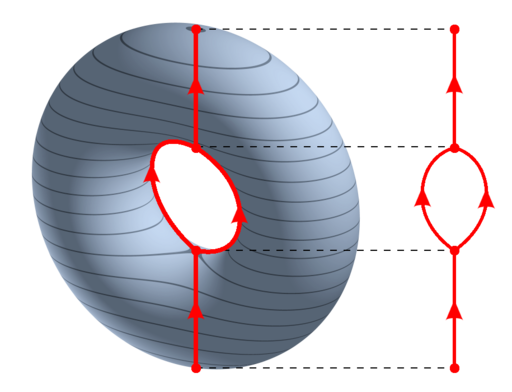
\includegraphics[width=0.4\textwidth]{3D-Leveltorus-Reebgraph.png}
	\caption{A Reeb graph of the torus.}
	\label{fig:reebgraph}
\end{figure}
\begin{figure}[htbp!] 
	\centering    
	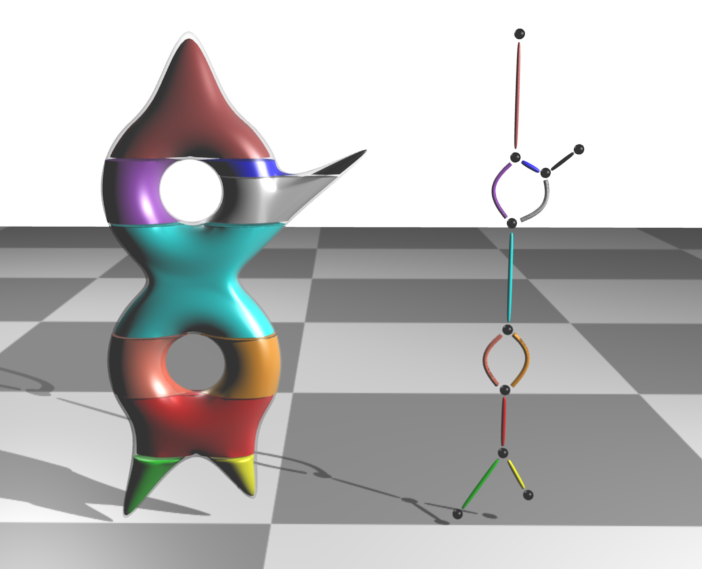
\includegraphics[width=0.4\textwidth]{reebgraph.png}
	\caption{A Reeb graph of the double torus. Image taken from \cite{reebgraphs}}
	\label{fig:reebgraph2}
\end{figure}

In figure \ref{fig:reebgraph} the topological space $(X,\mathcal{T})$ is the torus, and the function $f$ is the height function. The horizontal "slices" are the level sets of the torus with respect to $f$. The Reeb graph keeps track of the changes of the connected components of the level sets providing an effective representation of the torus. The Reeb graph can be thought as the skeleton of the topological space $(X,\mathcal{T})$, where the connected components of the level sets collapse into a point providing a condensed, summarized representation of the original space $X$. Another example can be seen in \ref{fig:reebgraph2}.

\subsection{Simplices and Simplicial Complexes}
In the example discussed in section 1.2, we saw that the output of Mapper was an undirected graph. This was only a simple case; the output of Mapper is a higher dimensional object, called \textit{simplicial complex}. We are interested in simplicial complexes because by the means of a suitable cover of the space $X$, the Nerve theorem \ref{nerve} provides a way to construct a simplicial complex that is homotopy equivalent to $X$. The outline of this section is the following: first we'll provide the reader with a purely combinatorial notion of a simplicial complex.  We'll provide an example to better illustrate this concept. Then, we'll introduce the concept of \textit{realization of a simplicial complex} in a vector space, that will further help the reader familiarize with this concept since it provides a more intuitive visualization of the simplicial complex. 

\begin{definition}{[\textit{Simplicial Complex}]}
	Given a finite set $X$, a \textbf{ simplicial complex} $\mathcal{K}$ on $X$ is a collection of subsets of $X$ such that:
	\begin{itemize}
		\item every singleton of $X$ is in $\mathcal{K}$ i.e. $\{x\} \in \mathcal{K}$ for every $x \in X$
		\item if $\gamma \subset X$ is in $\mathcal{K}$, then every subset of $\gamma$ must be in $\mathcal{K}$ as well.
	\end{itemize}
	Each $\gamma \in \mathcal{K}$, $\gamma \subset X$   is called \textbf{simplex} of dimension $|\gamma|-1$, where $|\gamma|$ is the cardinality of the subset $\gamma$ .
	\label{def:abstract_simplicial_complex}
\end{definition}

\begin{figure}[htbp!] 
	\centering    
	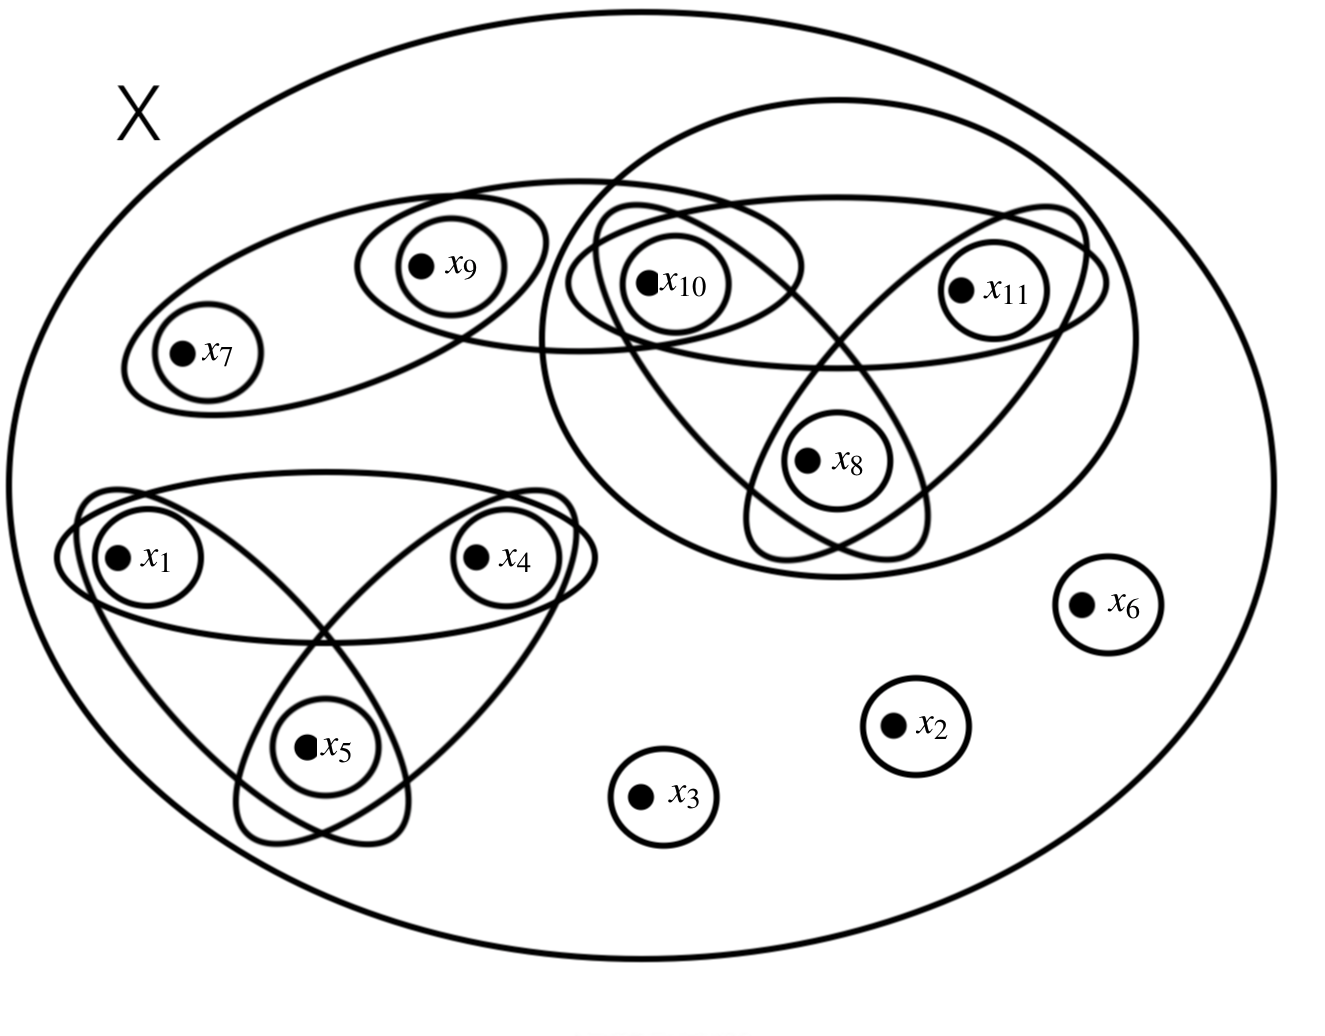
\includegraphics[width=0.5\textwidth]{abstract_simplicial_complex.png}
	\caption{A visualization of a possible collection of subsets of $X$ that satisfy the definition \ref{def:abstract_simplicial_complex} of \textit{abstract simplicial complex} on the finite set $X$ }
	\label{fig:abstract_simplicial_complex}
\end{figure}

In figure \ref{fig:abstract_simplicial_complex} we provide an example of a simplicial complex on the set $X=\{x_i, i=1,2, ...,11\}$. The elements of the abstract simplicial complex in figure \ref{fig:abstract_simplicial_complex} are: 
\begin{itemize}
	\item the 11 singletons $\{x_i\}, i=1,2, ..., 11$, called \textit{simplices} of dimension 0.
	\item the \textit{simplices} $\{x_1, x_4\}, \{x_4, x_5\}, \{x_5, x_1\}, \{x_7, x_9\}, \{x_9, x_{10}\}, \{x_{11}, x_{10}\}, \{x_8, x_{10}\}, \{x_8, x_{11}\}$  of dimension 1.
	\item the \textit{simplex} $\{x_8, x_{10}, x_{11}\}$ of dimension 2.
\end{itemize}

A few more useful definitions:
\begin{definition}{[\textit{n-face}]}
	Every simplex $\sigma$ of dimension $n$ which is a subset of a higher-dimensional simplex $\gamma$ is called \textbf{n-face} of the simplex $\gamma$.
	\begin{itemize}
		\item the \textit{0-faces} are called \textit{vertices}
		\item the \textit{1-faces} are called \textit{edges}
	\end{itemize}
\end{definition}
\begin{definition}{[\textit{facet}]}
	A \textbf{facet} is a simplex which is not the \textit{face} of any other higher-dimensional simplex
\end{definition}
The \textbf{dimension of a simplicial complex} is the largest dimension of any of its faces. A simplicial complex is said to be a \textbf{homogeneous $K$-complex} if any of its \textit{facets} has the same dimension $K$.
Let's continue the example in figure \ref{fig:abstract_simplicial_complex}. We can now see that the complex represented is a \textit{2-dimensional complex}, since its largest \textit{facet} has dimension 2. The \textit{1-faces} (or \textit{edges}) of the two-dimensional simplex $\{x_8, x_{10}, x_{11}\}$ are the three one-dimensional simplices $\{x_{11}, x_{10}\}, \{x_8, x_{10}\}, \{x_8, x_{11}\}$ and its \textit{vertices} are the zero-dimensional simplices $\{x_8\}, \{x_{10}\}, \{x_{11}\}$.\newline
It is useful to get a more geometric representation of a simplicial complex. To do so, we'll now build what is called the \textbf{realization of a simplicial complex} in a vector space.

\begin{definition}{[\textit{linearly independent points}]}
	The points $\{v_i\}_{i=0}^m \subset \mathbb{R}^n, 1\leq m\leq n$ are said to be \textbf{linearly independent} if the $m$ vectors $\{v_i-v_0\}_{i=1}^m$ are linearly independent.
\end{definition}
\begin{definition}{[\textit{convex hull}]}
	Given a set of points  $V = \{v_i\}_{i=1}^m \subset \mathbb{R}^n$, the \textbf{convex hull} of $V$ is the set of the convex linear combinations of the elements of $V$: $$ \{\sum_{i=1}^m{t_iv_i}\ :\ \sum_{i=1}^m{t_i}=1\}$$ 
\end{definition}
\begin{definition}{[\textit{realization}]}
	Given a finite set $X$ and an $K$-dimensional simplicial complex $\mathcal{K}$ on $X$, choose $\{v_x\}_{x\in X}$ linearly independent points in $\mathbb{R}^K$. The \textbf{realization of $\mathcal{K}$} is the union of the convex hulls of $\{v_x\}_{x\in \gamma}$ for every  simplex $\gamma\in\mathcal{K}$																														
\end{definition}

In figure \ref{fig:simplicial_complex} we provide a realization of the simplicial complex represented in figure \ref{fig:abstract_simplicial_complex}. The 2-simplex is represented by a triangle (the convex hull of three independent points in $\mathbb{R}^2$), the 1-simplices are represented by segments (the convex hulls of two independent points in $\mathbb{R}^2$) and the vertices are represented by simple points.
\begin{figure}[htbp!] 
	\centering    
	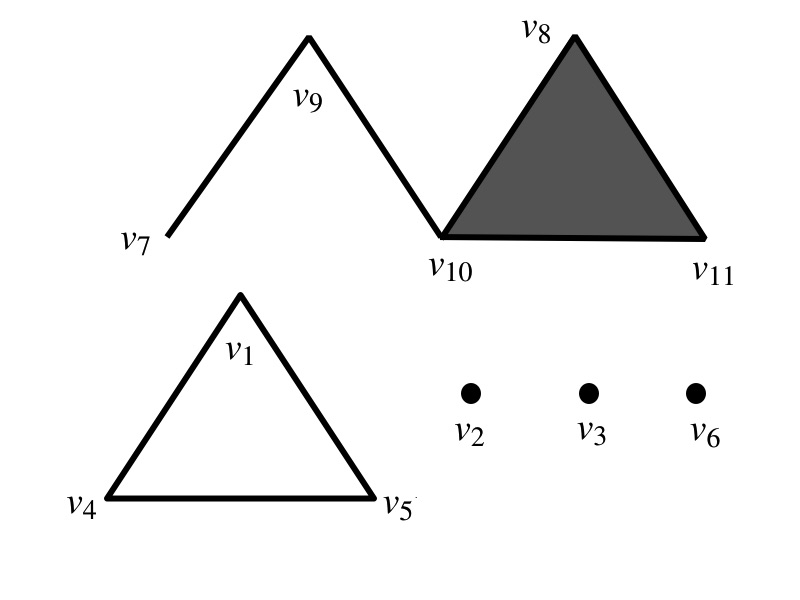
\includegraphics[width=0.5\textwidth]{simplicial_complex.jpg}
	\caption{A possible realization of the simplicial complex in figure  \ref{fig:abstract_simplicial_complex} }
	\label{fig:simplicial_complex}
\end{figure}

\begin{definition}{[\textit{nerve complex}]}
	Given a finite cover $\mathcal{A} = \{A_i\}_{i \in I}$ of a topological space $X$, its \textbf{nerve complex} is a simplicial complex $N(\mathcal{A})$ on the set $I$ of indices where $$N(\mathcal{A}) = \left\{J\subset I\colon\bigcap_{j\in J} A_j\neq \varnothing\right\}$$
\end{definition}

\paragraph{Example}
\begin{figure}[htbp!] 
	\centering    
	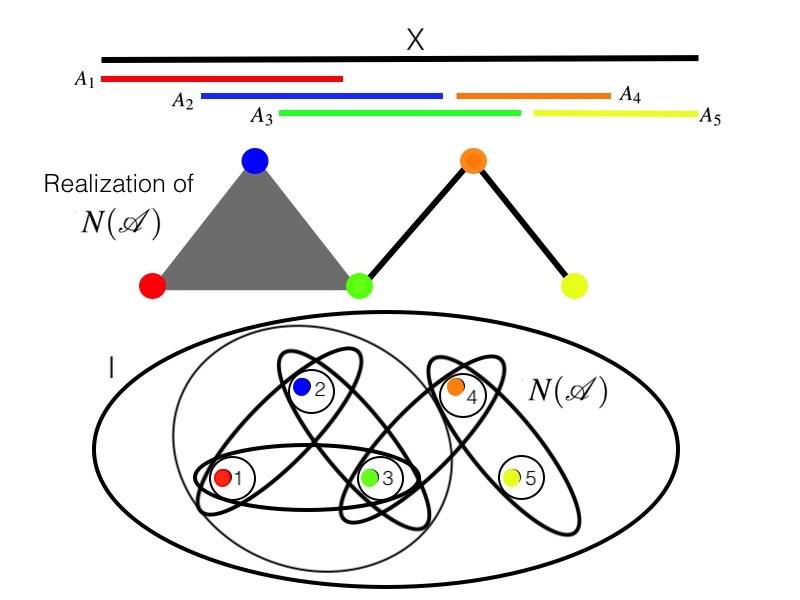
\includegraphics[width=0.5\textwidth]{nerve.png}
	\caption{the simplicial complex $N(\mathcal{A})$, nerve of the open cover $\{A_i\}$ of the set $X$ }
	\label{fig:nerve}
\end{figure}

Take the set $X$ as the segment in figure \ref{fig:nerve}, and as open cover $\mathcal{A}$ of $X$ the subsets $A_1,\  A_2,\  A_3,\  A_4,\  A_5$ $$ X = \bigcup_{i \in I}A_i , \  I = \{1, 2, 3, 4, 5\}$$ The \textit{nerve} of such a cover is the complex $N$ illustrated both in its combinatorial form and in its realization. We can observe that there are five \textit{1-dimensional simplices} (or \textit{edges}), one for every couple of subsets $A_i$ in the cover that overlap: $(A_1, A_2)$, $(A_2, A_3)$, $(A_1, A_3)$, $(A_3, A_4)$, $(A_4, A_5)$. Furthermore, the subsets $A_1, A_2, A_3$ all overlap i.e. $A_1 \cap A_2 \cap A3 \neq \varnothing$, and this leads to the creation of one \textit{2-dimensional simplex} with vertices the three subsets. In the realization of the nerve complex, the triangle represents the 2-dimensional simplex and the five edges (three edges of the triangle plus the two other edges)  represent the 1-dimensional simplices.

\paragraph{The Nerve Theorem}
From an open cover $\mathcal A=\{A_i\}_{i\in I}$ of the topological space $X$ it is possible to construct  a simplicial complex on the index set $I$ that is an "approximation" of $X$. 

\begin{definition}{[\textit{nerve of a cover}]}\\
	For a topological space $X$ and its covering $\mathcal A =\{A_i\}_{i\in I}$ we call nerve of the cover the simplicial complex on $I$: $$N(X,\mathcal{A}) = \left\{J \subset I\ |\ \bigcap\limits_{i\in J} A_i \neq \emptyset\right\}$$ 
\end{definition}

An important property, called the Nerve theorem, states that under a specific condition on the cover $\mathcal A$, the nerve $N(X, \mathcal A))$ is homotopy equivalent to $X$.

\begin{prop}[Nerve Theorem]
	Let $\mathcal A =\{A_i\}_{i\in I}$ be a open cover of a topological space X, if the following property holds
	$$\forall J\subset I \ \bigcap\limits_{i\in J} A_i \text{ is either empty or contractible to a point}$$
	then the nerve $N(X,\mathcal{A})$ is homotopy equivalent to $X$.
\end{prop}

Homotopy equivalent spaces have the important property of sharing the same "shape", or better, the same homology (\textit{Munkres, }\cite{Munkres}). In other words, the Nerve theorem tells us that, for a dataset $X$ sampled from a topological space $\mathcal O$ and a suitable open cover $\mathcal A$ of $X$ , the shape (homology) of the nerve $N(X,\mathcal A)$ is the same of the one of the ideal space $\mathcal O$.



\subsection{Mapper}
\label{sec:mapper}
The output of Mapper is a simplicial complex that can be thought as the skeleton of the abstract object $O$ from which the data point cloud $(X,d)$ is sampled. We saw how the Reeb graph is capable of providing an effective skeletonization of a space; Mapper can be thought as a pixelized version of the \textit{Reeb graph}, in the sense that Mapper provides an \textit{approximated} skeleton of the data point cloud $(X,d)$. Taking inspiration from \cite{multiscaleMapper}, hereunder we define a general construction,that illustrates the idea behind Mapper. We call this construction pixelized Reeb graph.
\begin{definition}{[\textit{pixelized Reeb graph}]}
	Let $(X,\mathcal{T})$ and $(Y,\mathcal{T}')$ be topological spaces and let $f : (X,\mathcal{T}) \rightarrow (Y,\mathcal{T}')$ be a well-behaved and continuous map. Let $\mathcal{B}=\{B_i\}_{i\in I}$ be a finite open cover of $Y$. The \textbf{pixelized Reeb graph} arising from these spaces is defined to be the nerve simplicial complex of the connected components of the pullback cover.
	\label{def:pixelizedreebgraph}
\end{definition}
\begin{remark}{(on definition \ref{def:pixelizedreebgraph})}
	Consider $(X,\mathcal{T})$ a topological space and $f:(X,\mathcal{T})\rightarrow\mathbb({R},\mathcal{T}')$, where $\mathcal{T}'$ is the metric topology. Then consider the following option for $\mathcal{B}=\{B_{\alpha}\}_{\alpha\in A}$: $B_\alpha = (\alpha-\epsilon,\alpha+\epsilon)$ for $\alpha\in A=\{k\epsilon'\}_{k\in Z}$, $\epsilon'\in(0,2\epsilon)$ for some fixed $\epsilon>0$. This correspond to "$\epsilon$-thick level sets", which induce a relaxed notion of Reeb graphs.
\end{remark}

In other words: given a topological space $(X, \mathcal{T})$ we map it through a continuous function $f$ in $(Y, \mathcal{T}')$. Then, we define a cover $\mathcal{B}$ of $Y$ and we obtain the pullback cover $\mathcal{A} = \{ A_i \}_{i \in I}$ on $X$. Then for each subset $A_i \in \mathcal{A}$ we take its partition $  \{ A_i^{(j)}  \}_{j \in J_i}$ made by its connected components, whose existence is assured by theorem \ref{theo:connected_components}. We build then the nerve complex of the pullback cover split into its largest connected subspaces i.e. $N( \{A_i^{(j)}, i \in I, j \in J_i\} )$\newline
A data point cloud $X$ can be thought of as sampled from an underlying space with a particular shape that we are interested to capture and visualize through a process as close as possible to the pixelized Reeb graph. To do so, we need a similar notion of connected subspace but for a data point cloud. To do so we use a common clustering algorithm for metric spaces, the \textit{simple linkage algorithm}. The clusters obtained will be our "connected components". Linkage algorithms depend on a parameter $\epsilon$ fixed \textit{a priori}; different choices of this parameter lead to different partitions of the data point cloud. The smaller $\epsilon$, the more this notion of connectedness is strong, and the more the algorithm will lead to the creation of many but small clusters. On the contrary, the bigger $\epsilon$, the more relaxed the notion of connectedness and the more the algorithm creates few but bigger clusters. The output of Mapper will be sensible to changes of this parameter, that needs to be suitably tuned.

\begin{definition}{[\textit{Single Linkage algorithm, connected components in a metric space}]}
	Fix a positive real number $\epsilon>0$. An $\epsilon$-path in $X$ is a set $$P_\epsilon\ =\ \{x \in X\ :\forall x_0,x_n\in P_\epsilon\  \exists \{ x_1, x_2, ..., x_{n-1}\} \subset P_\epsilon: d(x_i,x_{i+1})<\epsilon\  \forall i = 0, ..., n-1\}$$ Two points $x,y$ in the data point cloud $(X,d)$ belong to the same cluster (or "connected component") if there exists an $\epsilon$-path that connects the two i.e. $\exists \ P_\epsilon\ :\ x,y\in P_\epsilon$
	\label{def:connected_component_metric}
\end{definition}
Now that we have this notion of connectedness for metric spaces, we can modify slightly the definition \ref{def:pixelizedreebgraph} to have Mapper:
\begin{definition}{[\textit{Mapper}]}
	Let $(X,d)$ be a data point cloud and $(Y,\mathcal{T}')$ be a topological space. Let $f : (X,\mathcal{T}) \rightarrow (Y,\mathcal{T}')$ be a continuous map, where $\mathcal{T}$ is the metric topology. Let $\mathcal{B}=\{B_i\}_{i\in I}$ be a finite open cover of $Y$. Fix a real parameter $\epsilon>0$ for the single linkage algorithm. The \textbf{Mapper construction} arising from these data is defined as the simplicial complex induced by the nerve of the connected components $A_i^{(j)}$ (in the sense of definition \ref{def:connected_component_metric}) of the pullback cover $\mathcal{A}=\{A_i\}_{i\in I}\ =\ f^{-1}(\mathcal{B})$ $$M(X,d,\epsilon,f,\mathcal{B})\ =\ N(\{A_i^{(j)}\})$$
\end{definition}

Before moving to an example, it must be specified that in this section we used the single linkage algorithm to define a notion of connectedness in metric spaces; any other kind of clustering algorithm can be used, as soon as it leads to a partition of each element of the pullback cover $\mathcal{A}$. Some options could be other linkage algorithms, such as complete linkage and average linkage algorithms \cite{InformationRetrieval}. 

\subsubsection {Example}
We present an example of application of Mapper, where the typical choice of parameters is used. Furthermore, we discuss the importance of a correct choice of the $\epsilon$ parameter in the simple linkage algorithm.
To summarize the choice of parameters for this example,
\begin{itemize}
	\item $X \subset \mathbb{R}^2$ is the data point cloud represented in figure \ref{fig:epsilon} sampled from a circle with some noise.
	\item  $Y=\mathbb{R}$ endowed with the euclidean metric topology. 
	\item $d$ is the usual euclidean metric in $\mathbb{R}^2$
	\item $f : X \rightarrow \mathbb{R}$ is the height function $(x,y) \rightarrow y$
	\item $\mathcal{B}$ is the cover set by the colored intervals in figure \ref{fig:epsilon} $$\mathcal{B} = \{B_1=(b3,+\infty),\ B_2=(b_1,b_4),\ B_3=(-\infty,b_2)\} \text{ where } b_1<b_2<b_3<b_4$$
	\item $\epsilon$ varies
\end{itemize}
Let's consider a data point cloud $(X,d) \subset \mathbb{R}^2$ represented in figure \ref{fig:epsilon}. We consider the usual euclidean distance $d$, as filter function $f:X\rightarrow\mathbb{R}$ the usual height function, and as cover $\mathcal{B}$ the cover given by the three colored overlapping intervals in figure \ref{fig:epsilon}. We represent the pullback cover by coloring the points by the same color of the interval that they are mapped to. Points that are mapped by $f$ on a value belonging to an overlapping zone, are colored by both colors of the corresponding overlapping intervals. We represents clusters by explicitly drawing one of the possible $\epsilon$-path.
In figure (a) $\epsilon$ was chosen too small: the result is that the green point at the bottom is too far form the other green points and so it gets clustered alone, it's not considered "connected" to the other green points. Figure (b) is a "good" approximation of a circle: the linkage algorithm led to an intuitive clustering of the data point cloud, where all the green points are considered connected together, as well as all the blue ones. The violet points are grouped in two distinct clusters: the points on the left and the points on the right, since it is impossible to find a violet point on the left that is less than $epsilon$ away to any of the violet points on the right. If we choose an $\epsilon$ big enough that it is possible to find a violet point on the left and a violet point on the right that are less than epsilon away, all the violet points will be considered "connected" i.e. belonging to the same cluster. This will make the Mapper look like a straight line, loosing any information about the hole in the middle of the data point cloud.


\begin{figure*}[!htbp]
	\centering
	\begin{subfigure}[t]{0.4\textwidth}
		\centering
		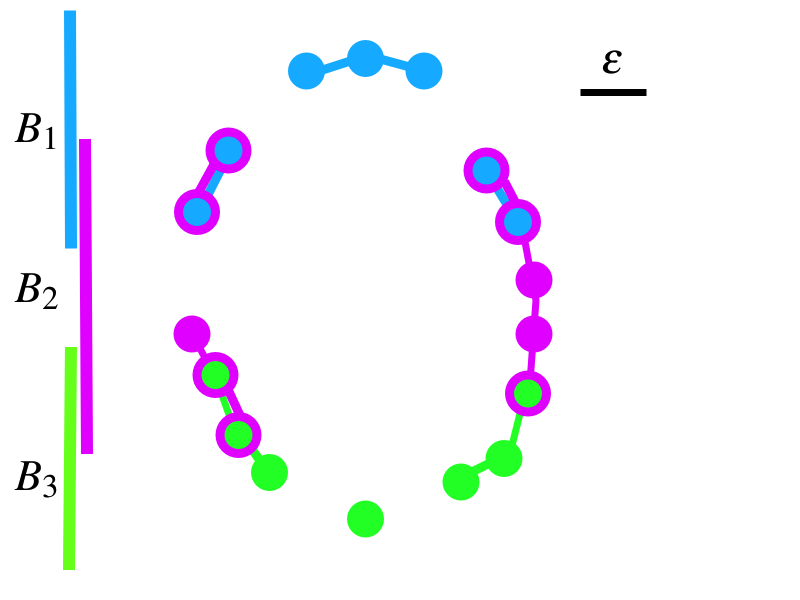
\includegraphics[height=1.5in]{torus_approximation_small_colored.png}
		
	\end{subfigure}
	~ 
	\begin{subfigure}[t]{0.4\textwidth}
		\centering
		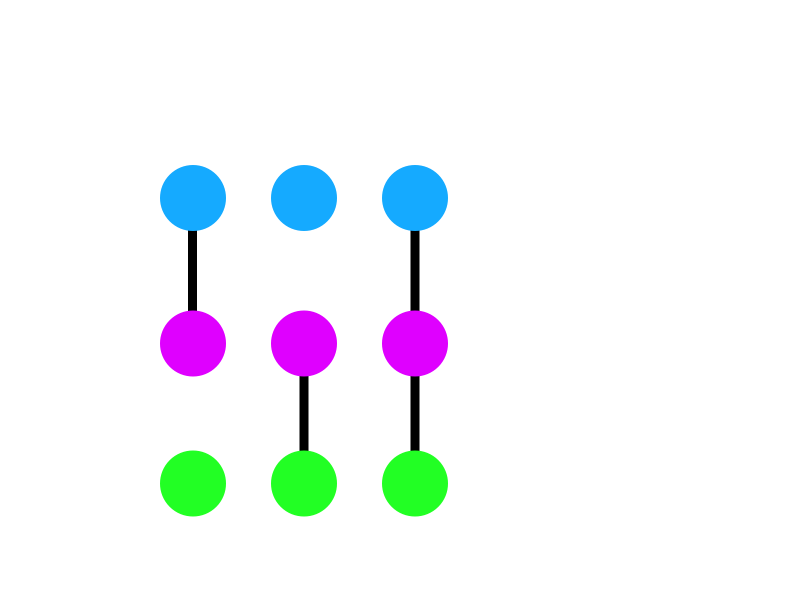
\includegraphics[height=1.5in]{mapper_of_torus_small.png}
		
	\end{subfigure}
	
	~ 
	\begin{subfigure}[t]{0.4\textwidth}
		\centering
		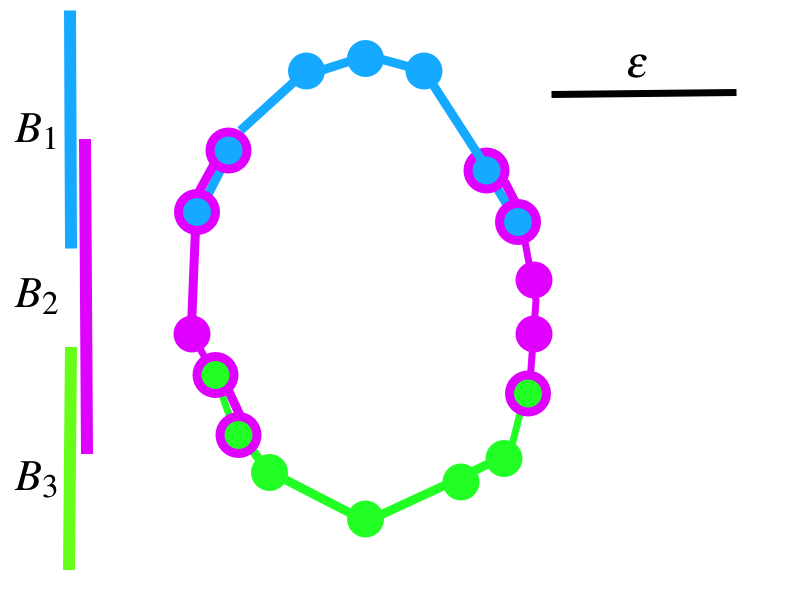
\includegraphics[height=1.5in]{torus_approximation_colored.png}
		
	\end{subfigure}
	~ 
	\begin{subfigure}[t]{0.4\textwidth}
		\centering
		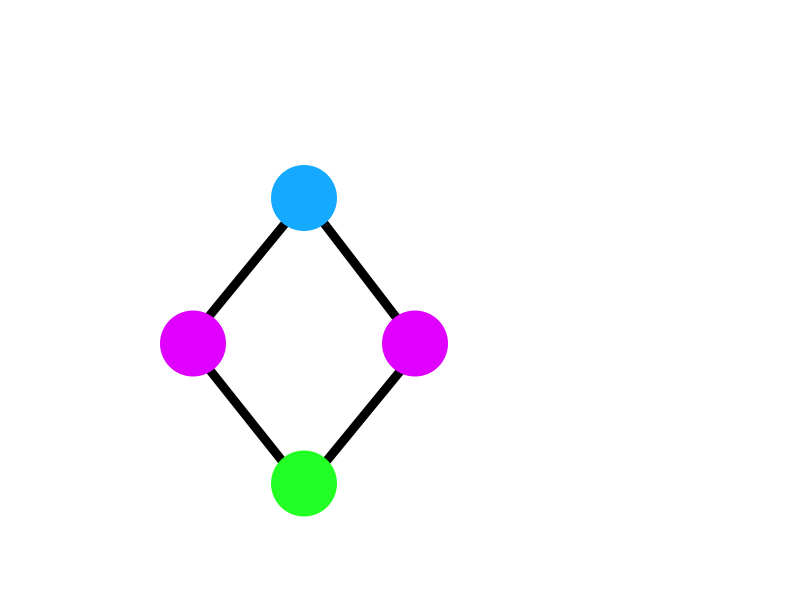
\includegraphics[height=1.5in]{mapper_of_torus.png}
		
	\end{subfigure}
	\centering
	
	~ 
	\begin{subfigure}[t]{0.4\textwidth}
		\centering
		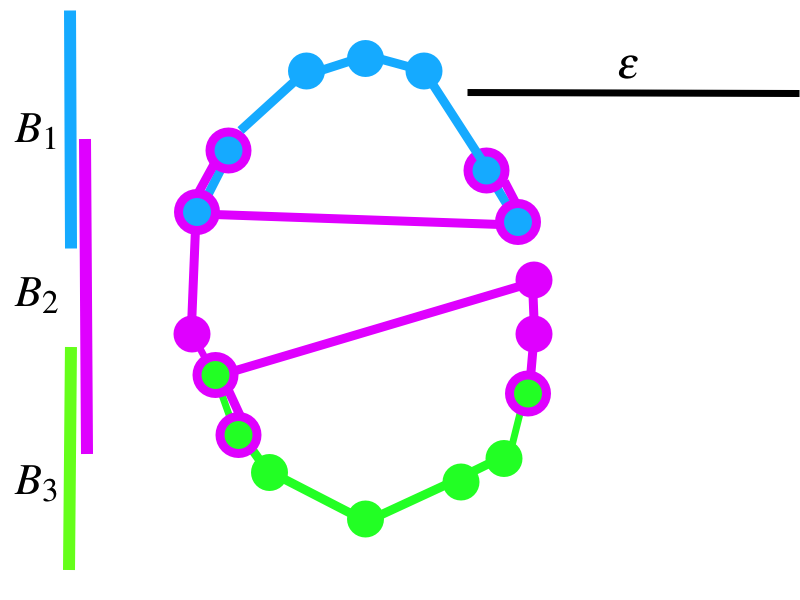
\includegraphics[height=1.5in]{torus_approximation_big_colored.png}
		
	\end{subfigure}
	~ 
	\begin{subfigure}[t]{0.4\textwidth}
		\centering
		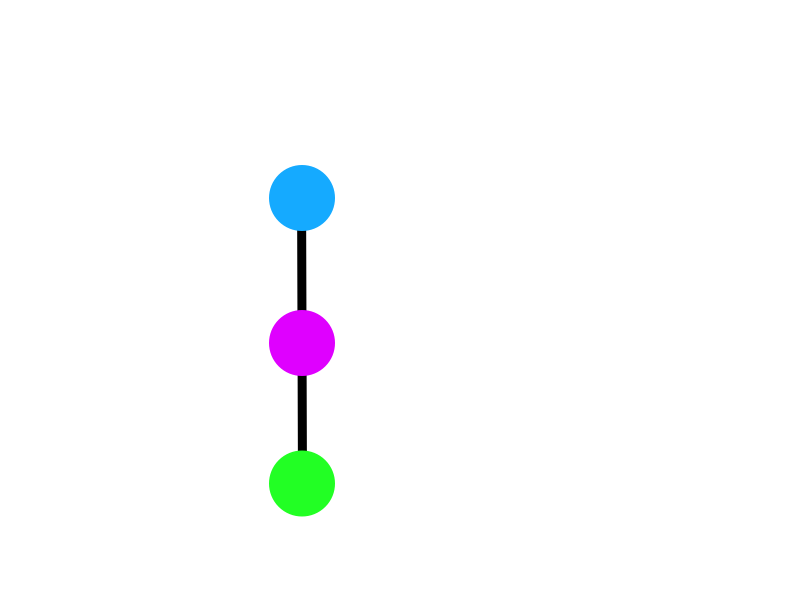
\includegraphics[height=1.5in]{mapper_of_torus_big.png}
		
	\end{subfigure}
	\caption{different choices of $\epsilon$ lead to different Mappers.}
	\label{fig:epsilon}
\end{figure*}

Playing with toy examples like this it is possible to understand what happens in many different configurations of the parameters $(d, f, \mathcal{B}, \epsilon)$ of Mapper. Many different configurations lead indeed to many different outputs. In the next section some choices for these parameters common in literature are presented.

\subsubsection{Selection of parameters}
In this subsection the cover $\mathcal{B} = \{B_i\}_{i \in I}$ is assumed to be built by $n$ equally spaced, overlapping intervals $B_i$. Only the dependence of Mapper on the distance $d$, on the filter function $f : X \rightarrow \mathbb{R}$ and on $\epsilon$ is developed. Common choices of $d$, $f$ and $\epsilon$ made in practical applications found in \cite{extracting_insights}\cite{PAD} are discussed.
\subsubsection{Filter function}
\paragraph{Geometric filters} It is common to use filter functions that depend only on the distance $d$. Such filters $f: (X,d) \rightarrow \mathbb{R}$ are often a measure of the local density of the data point cloud or a measure of a centrality of the point $x$. One typical example of centrality measure is the $L_\infty$-centrality $f_\infty$: $$ f_\infty (x) = \max _{y\in X}d(x,y) $$
High values of $f$ correspond to points "far" from the center of the data point cloud; the level sets $f^{-1}(B_i)$ will be consequently made by points at about the same "distance" from the center of the point cloud.  Filters that depend only on the distance $d$ are called \textit{geometric filters}. \newline 
\paragraph{More filters}
On the other hand, a possible choice is to take as filter $f_P: (X,d)\rightarrow\mathbb{R}$ the projection of the points on one direction of choice. This was the choice made in the introductory example, where $f$ was chosen as the projection on the first coordinate of the points $x\in\mathbb R^3$. Consider the data matrix $X\in\mathbb{R}^{m\times n}, n>m$, where each column is made by the vector of the $m$ components of the corresponding data point $x$. The most common direction onto which to project the data point cloud is the first principal direction of the data matrix $X$: to get an intuition of why this could be a good choice, consider the following reasoning. \newline 
Any matrix $X$ can be decomposed in its singular value decomposition $$X=USV^T$$ where $U$ is an $m \times m$ unitary matrix, $S$ is a $m \times n $diagonal matrix and $V$ is an $n\times n$ orthonormal matrix. The column vectors of $V$ are called principal directions of $X$. Imagine that the data points are generated in an i.i.d. fashion from some distribution $\mathcal{D}_X$. Assume that we have preprocessed the data to subtract the mean from each row. The empirical covariance $K$ is given by 
$$n\cdot K=\sum_{i=1}^{n}x_ix_i^T = XX^T=USV^TVS^TU^T=USS^TU^T=US_m^2U^T$$ where $S_m$ is the $m\times m$ diagonal matrix consisting of the $m$ first columns of $S$. Consider the linear transformation of the features $\hat{X}=U^TX$. The empirical covariance $\hat{K}$ is given by 
$$n\cdot \hat{K}=\hat{X}\hat{X}^T=U^TXX^TU=U^TUS^2U^TU=S_m^2$$
This means that $\hat{X}$ is a linear transformation of the features such that the empirical covariance $\hat{K}$ is diagonal i.e. the transformed features are uncorrelated. Furthermore, the first transformed feature is the one with the highest variance, given by the square of the first singular value divided by $n$: $\frac{1}{n}\cdot(S)_{1,1}^2$. From this point of view, the intuition of why projecting on the first principal component could be a good idea is the following: to each point $x$, the filtered value $f_P(x)$ represents the value of the component of $x$ with the highest variance in the linearly transformed, uncorrelated feature space.\newline
Another interpretation, less probabilistic but more geometric, is the following: one can imagine the first principal direction as the direction along which the data point cloud is distributed. In the introductory example, it was natural to project the "hand" on the $x$ axis since it was possible to see that the hand was aligned, or "pointing" in the x-direction. Such a choice makes the projections $f(X)\subset\mathbb R$ as spread along the real axis as possible (or, in the previous interpretation, with the highest variance as possible) and thus ease the process of finding a suitable cover $\mathcal{B}$.\newline
Another example of filter is the following: $f(x)=||x||_{L^p}^k$\cite{PAD}. This is a measure of how much a point is far from the origin, and it is useful when analyzing data that represent deviations form a normal value, centered in the origin. How to choose $p$ and $k$ is not clear however, and several experiments have to be made depending on the particular application to find the combination of $(p,k)$ that gives the best output.
\paragraph{} There is a high degree of arbitrariness in choosing an appropriate filter function. An advantage of geometric filters with respect to more general filters is their independence on the particular choice of coordinates used to represent the data matrix $X$. However, they introduce limited amount of information in the algorithm and they are limited to density and centrality measures since they depend only on the distance $d$.
\subsubsection{Clustering algorithm and $\epsilon$}
Our interpretation of clustering together two points consist in considering them to belong to the same "connected component" of the data point cloud. Any clustering algorithm could be used, however the most common in literature are the \textit{linkage algorithms}. Linkage is an algorithm where at each step clusters are merged together into bigger and bigger ones, until there are no clusters left closer to each other than a threshold $\epsilon$.
\begin{definition}{[\textit{Linkage Algorithm}]}
	Start with defining each element as a cluster on its own. Define a distance $d_L(A,B)$ between two clusters $A, B$. At each step, the two closest clusters are combined into one, until there are no more clusters close to each other by less than a threshold valued $\epsilon$.
\end{definition}
The choice of the cluster distance $d_L$ defines different kind of linkage algorithms. $d_L(A,B)=\min_{x\in A, y\in B}d(x,y)$ defines the \textbf{Single Linkage} algorithm; $d_L(A,B)=\max_{x\in A, y\in B}d(x,y)$ defines the \textbf{Complete Linkage} algorithm; $d_L(A,B)=\frac{1}{|A|\cdot|B|}\sum_{x\in A}\sum_{y\in B}d(x,y)$ defines the \textbf{Average Linkage} algorithm. Whatever choice is made on $d_L$, different methods can be chosen to determine $\epsilon$. Hereunder two possible methods are presented:
\begin{definition*}{[\textit{Histogram method}]}
	Given an integer $k$, create a histogram of $k$ equally spaced bins of the number of \textit{merges} of clusters as function of the threshold value $\epsilon$. Select $\epsilon$ to be the threshold corresponding to the first gap in the histogram. If no gap is observed, the parameter $k$ has to be chosen smaller until a gap is observed.
\end{definition*}
\begin{figure}[htbp!] 
	\centering    
	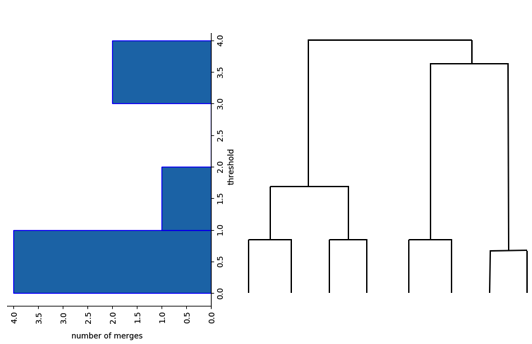
\includegraphics[width=0.5\textwidth]{histogram_method.png}
	\caption{The histogram method}
	\label{fig:histogram_method}
\end{figure}
An example is provided in figure \ref{fig:histogram_method}. On the right, the dendogram of a possible linkage is showed. On the left, the corresponding histogram with $k=4$ is build. In this example the threshold $\epsilon$ would then be set at the value $\epsilon=2$.

Notice that a high value of $k$ produces a finer histogram, and consequently the first gap will be observed with lower values of $\epsilon$.
\begin{definition*}{[\textit{Simple gap method}]}
	Proceed with the linkage algorithm chosen. Increase the threshold value linearly in time. As soon as for a fixed amount of time $\delta t$ new merges of clusters are not observed, the algorithm is stopped.
\end{definition*}

Notice that both methods need an extra parameter to be chosen, again. For the histogram method $k$ must be fixed, and for the single gap method $\delta t$ must be fixed. In conclusion, there is no unique way to properly fix $\epsilon$. Some experiments have to be made to find a suitable value for each particular case. Furthermore, there's no unique definition of "suitable": as saw in figure \ref{fig:epsilon}, it is hard to judge only by the corresponding different outputs of Mapper when $\epsilon$ is "well set". The choice of $\epsilon$ is ultimately left to the researcher, who has to try different methods, interpret the result and make a "reasonable" choice.
\subsubsection{Distance $d$}
In Mapper, the distance $d : X \times X \rightarrow \mathbb{R}$ intervenes \textit{only} in the clustering step of the level sets $f^{-1}(B_i)$. In all the definitions given until now $d$ was always referred to as a metric respecting the three axioms of definition \ref{def:metric}. However, to successfully execute any of the linkage algorithms described above, it can be observed that is not strictly necessary for $d$ to satisfy the axiom of identity of the indiscernibles i.e. $d(x,y)=0 \implies x=y$. A function $d:X\times X \rightarrow\mathbb{R}$ that satisfies only the properties of positivity and triangle inequality is called a \textbf{dissimilarity metric}. When adopting such a dissimilarity metric on $X$, two points $x,y$ belonging to the same level set such that $d(x,y)=0$ will always be clustered together, no matter the choice of $\epsilon$. This is useful to filter out some noise in the data. The \textit{mismatch distance} described in \cite{TwoTierMapper} that will be presented in Chapter 2 is an example of dissimilarity metric. When defining a dissimilarity metric on $X$ instead of a proper metric, all the definitions given previously in this section can be adapted consequently. \newline
In applications, the notion of metric can be relaxed even more. Indeed, one of the most used "distances" on $X$ is the Pearson correlation distance. By Pearson correlation distance one of the two following definitions can be chosen:
\begin{equation*}
d_{\text{Pearson, 1}} : (x,y)\rightarrow1-|\text{Corr}(x,y)|
\end{equation*}
\begin{equation*}
d_{\text{Pearson, 2}} : (x,y)\rightarrow1-\text{Corr}^2(x,y)
\end{equation*}
where $\text{Corr}(x,y)=\frac{s_{xy}}{s_xs_y}$ and $s_x,\ s_y$ are the sample standard deviations, and $s_{xy}$ is the sample covariance.
Notice that it is possible to come up with examples that prove that these definitions of distance do not respect even the triangle inequality.\newline





















\pagebreak

\section{Previous Implementations}
In this section we briefly describe the most used libraries at the moment that implement the Mapper algorithm. In particular, we focus on discussing their architecture and design choices, highlighting the corresponding pros and cons.

\subsection{Kepler Mapper}
\paragraph{Kepler Mapper}
Kepler Mapper is a pure Python implementation of the Mapper algorithm. It relies on clustering and filter functions implemented in the popular package Scikit-learn. However, compared to other implementations described further on, it is limited. It implements only one type of cover, and furthermore it does not compute the nerve of such cover, but only its one-dimensional skeleton. In other words, it completely ignores simplices with dimension $d, d>=1$. Such a one-dimensional skeleton is nothing else than a simple undirected graph.\\
As a filter function, the user can provide a Scikit-learn API compatible object (an object with a $fit\_transform()$ method) or a user-made numpy.ndarray containing the filter values of the data points. As a clustering algorithm, Kepler Mapper uses Scikit-learn API compatible clustering algorithms, that means a class with the following methods: get\_params(), fit(), and the following attribute: \_labels.

At the present Kepler Mapper is under constant development ( as at the 10th of March 2019 the GitHub repo has 482 commits, 8 branches, 6 releases, last published commit the 6th of March 2019).

Kepler Mapper implements a very effective visualization of the output graph. The package provides a base HTML file, and uses Jinja2 to modify such a base HTML file with the data contained in the output graph to produce a new HTML file that renders the output graph.
\paragraph{Architecture}
This package (as in September 2018) is implemented in an OOP fashion, and consists of only three classes: KeplerMapper, Cover, GraphNerve. Figure \ref{fig:keplermapper} illustrates this simple architecture. This architecture is really simple if compared to the more complex one of Python Mapper (a second implementation of Mapper) illustrated in figure \ref{fig:pymapper}.
\paragraph{Example}
We present an easy use-case example of this package, discussing how the steps of Mapper were implemented in the package.
\begin{lstlisting}[language=Python, caption=Kepler Mapper example]
# Import the class
import kmapper as km

# Some sample data
from sklearn import datasets
data, labels = datasets.make_circles(n_samples=5000, noise=0.03, factor=0.3)

# Initialize
mapper = km.KeplerMapper(verbose=1)

# Fit to and transform the data
projected_data = mapper.project(data, projection=[0,1]) # X-Y axis

# Create dictionary called 'graph' with nodes, edges and meta-information
graph = mapper.map(projected_data, data, nr_cubes=10)

# Visualize it
mapper.visualize(graph, path_html="make_circles_keplermapper_output.html",
title="make_circles(n_samples=5000, noise=0.03, factor=0.3)")
\end{lstlisting}
\begin{itemize}
	\item Step 1: evaluating the filter function $f$. \\The filter values $f(X)$ are calculated in line 12. Internally, the KeplerMapper object uses functions imported from Numpy and Scikit-Learn to calculate the projection on the x-y axis of the data points. The user is just requested to insert as arguments of the $project()$ method a list of indices identifying the axis onto which to project the data.
	\item Step 2: computing the pullback cover $\mathcal B$. \\This step is done in line 15. The default cover implemented in Kepler Mapper is a uniform cover with 10 intervals and a percentage of overlap of 20\%. The user can modify this clustering algorithm by passing to the method $KeplerMapper.map()$ a Scikit-learn API compatible clusterer in the following way:
	\begin{lstlisting}[language=Python]
from kmapper.cover import Cover
graph = mapper.map(projected_data, data, nr_cubes=10, coverer=Cover(nintervals=15, perc_overlap=0.4))\end{lstlisting}
	\item Step 3: clustering the pre images $\{B_i\}$.\\This step is done again in line 15. The default clustering scheme implemented in Kepler Mapper is DBSCAN, implemented in $sklearn.cluster.DBSCAN()$. The user can modify this clustering algorithm by passing to the method KeplerMapper.map() a Scikit-learn API compatible clusterer in the following way:
	\begin{lstlisting}[language=Python]
custom_clusterer = sklearn.cluster.DBSCAN(eps=0.5, min_samples=3)
graph = mapper.map(projected_data, data, nr_cubes=10, clusterer=custom_clusterer)\end{lstlisting}
	\item Step 4: building the nerve complex. \\This step is done again in line 15 and the nerve complex is stored as a Python dictionary returned by the method $KeplerMapper.map()$. Such Python dictionary has the following keys: "nodes", "links", "simplices", and "metadata" where $graph["links"]$ and $graph["simplices"]$ are return values of a call to a GraphNerve functor.
	\item Step 5: visualizing the graph.\\Line 18. $KeplerMapper.visualize()$ is a really interesting method. In 35 lines of code it converts the information contained in the graph dictionary to a very effective HTML/D3.js visualization thanks to Jinja templates. See \cite{KMapper} for the source code. See figure \ref{fig:keplermapperoutput} for an example.
\end{itemize}
\begin{figure}[h!]
	\caption{KeplerMapper Github statistics}
	\centering
	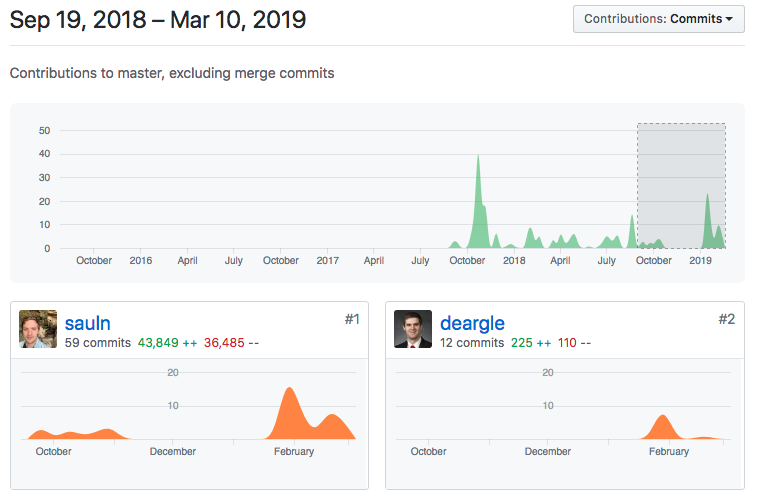
\includegraphics[width=0.8\textwidth]{images/keplermappergithubstats.png}
	\label{fig:keplermappergithubstats}
\end{figure} 
\begin{figure}[h!]
	\caption{KeplerMapper output example}
	\centering
	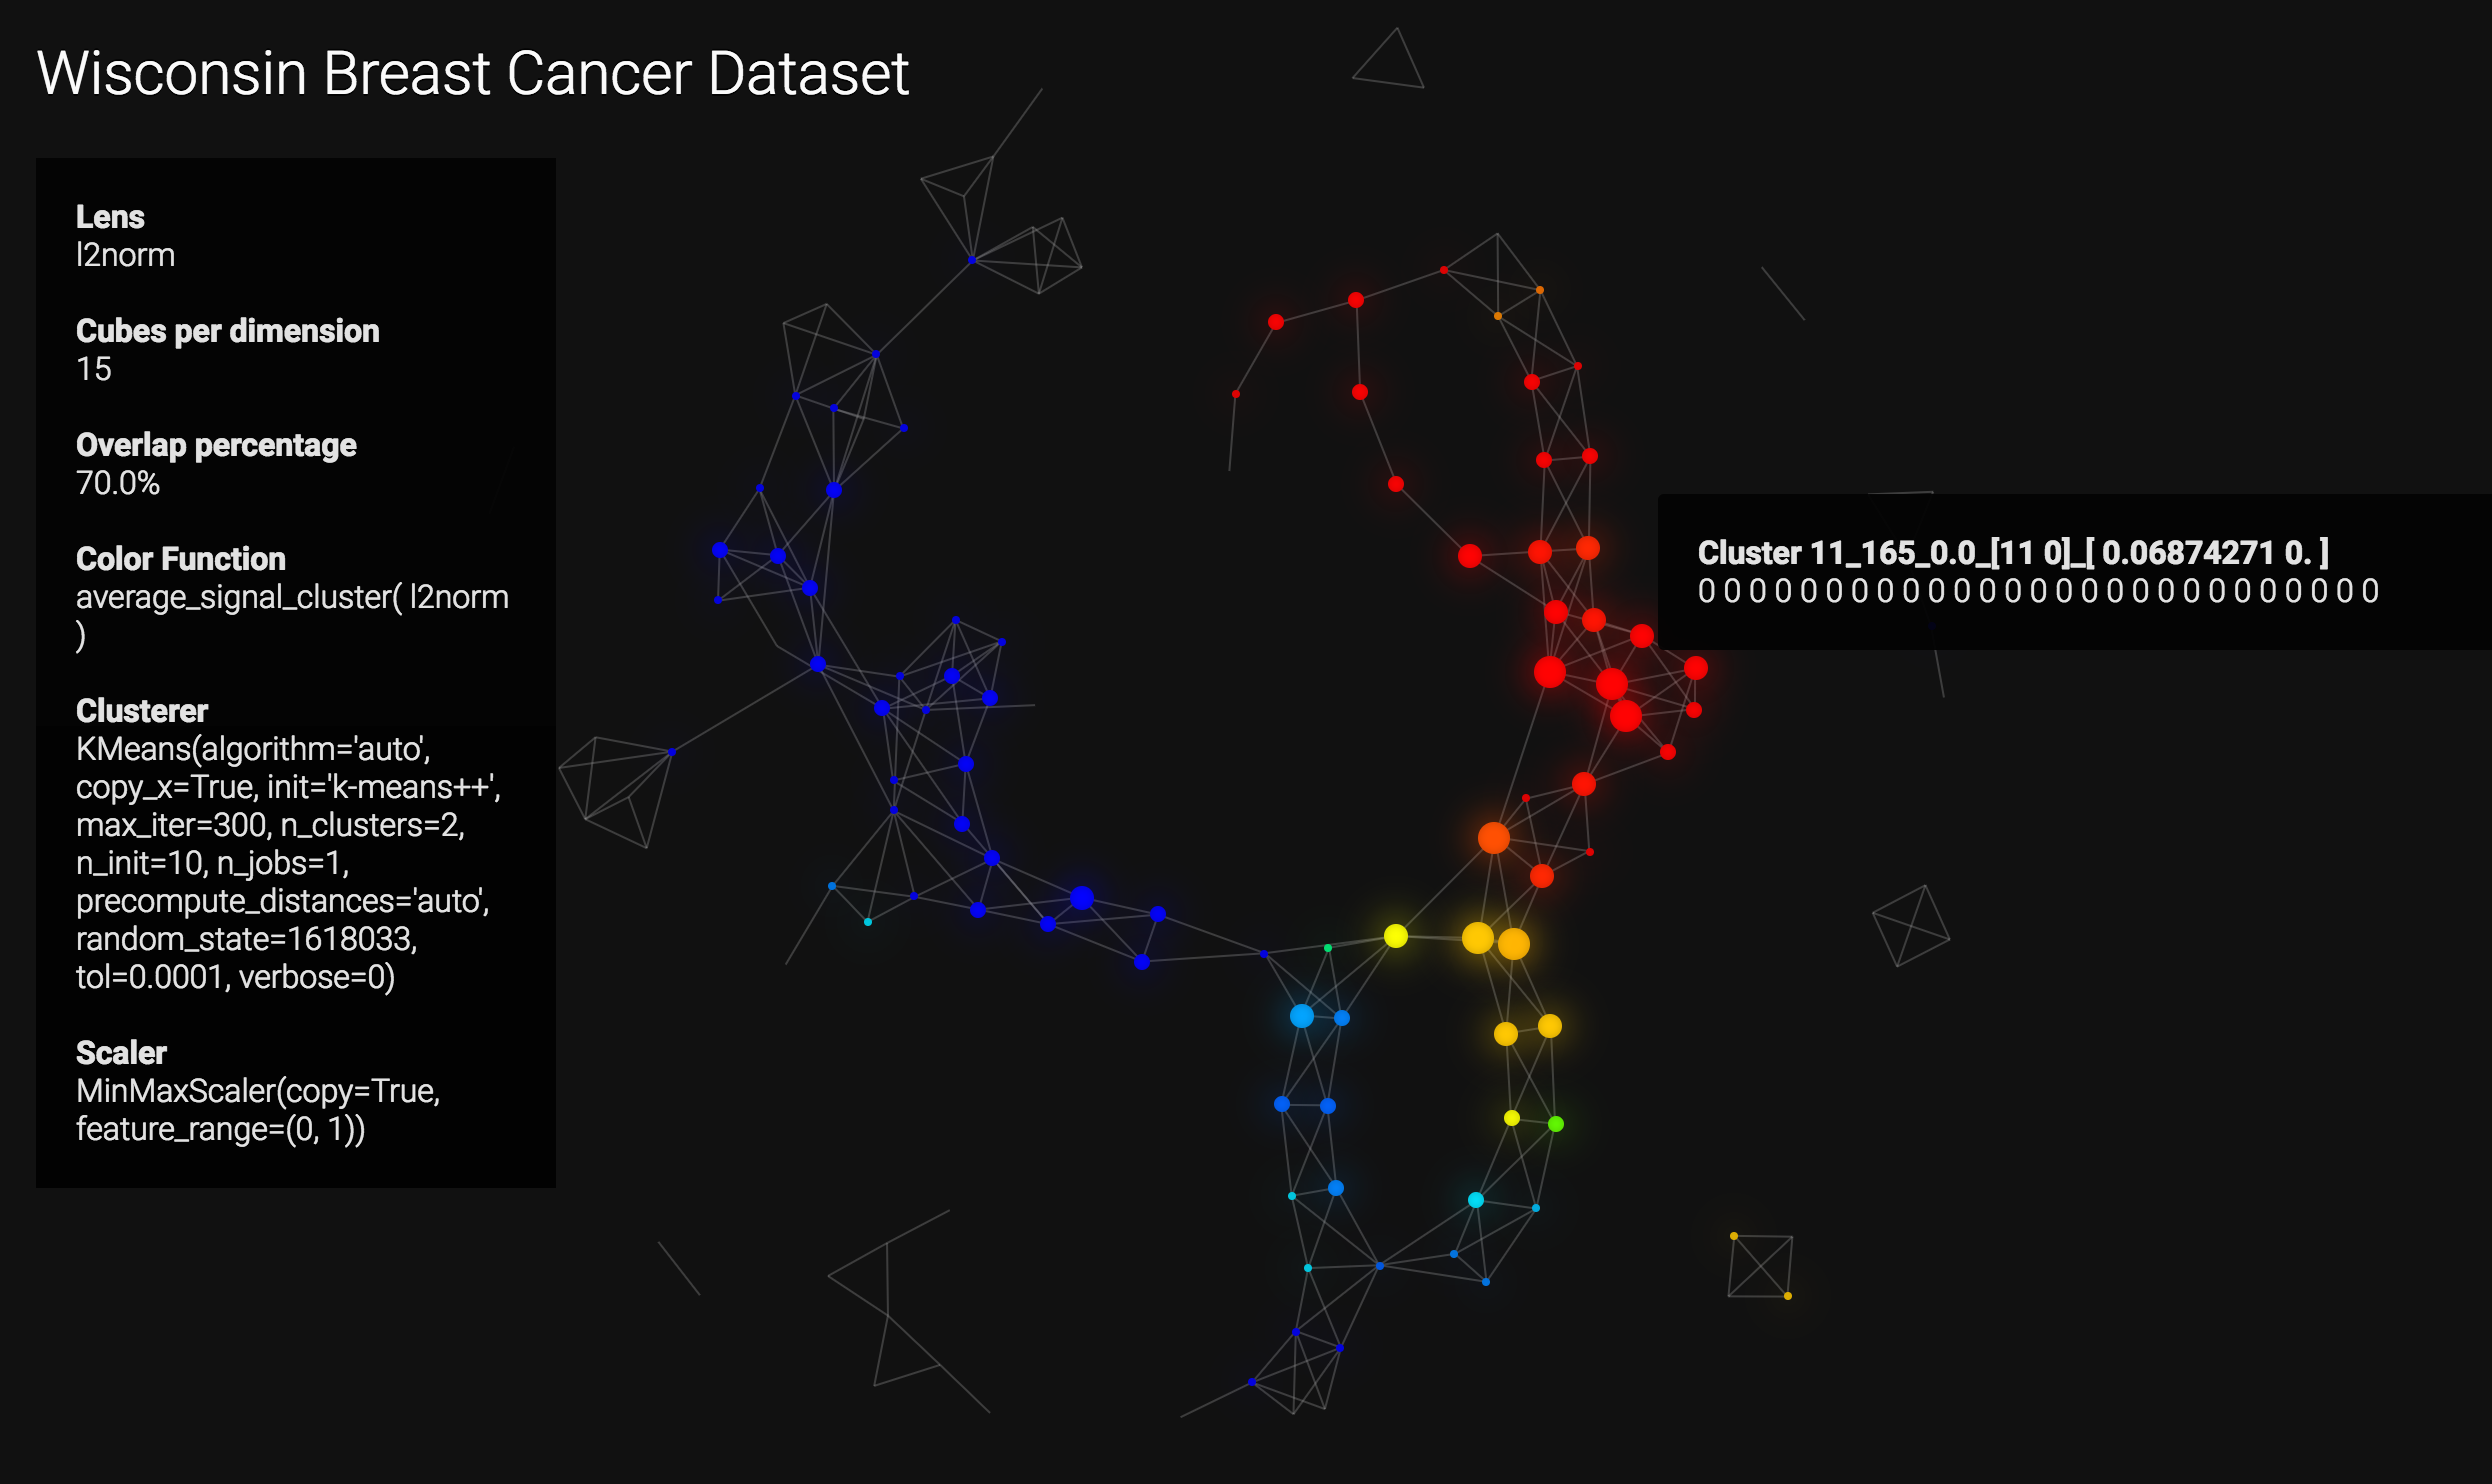
\includegraphics[width=0.8\textwidth]{images/keplermapper.png}
	\label{fig:keplermapperoutput}
\end{figure} 

\begin{figure}[h!]
\caption{Kepler Mapper Architecture (as in September 2018)}
\centering
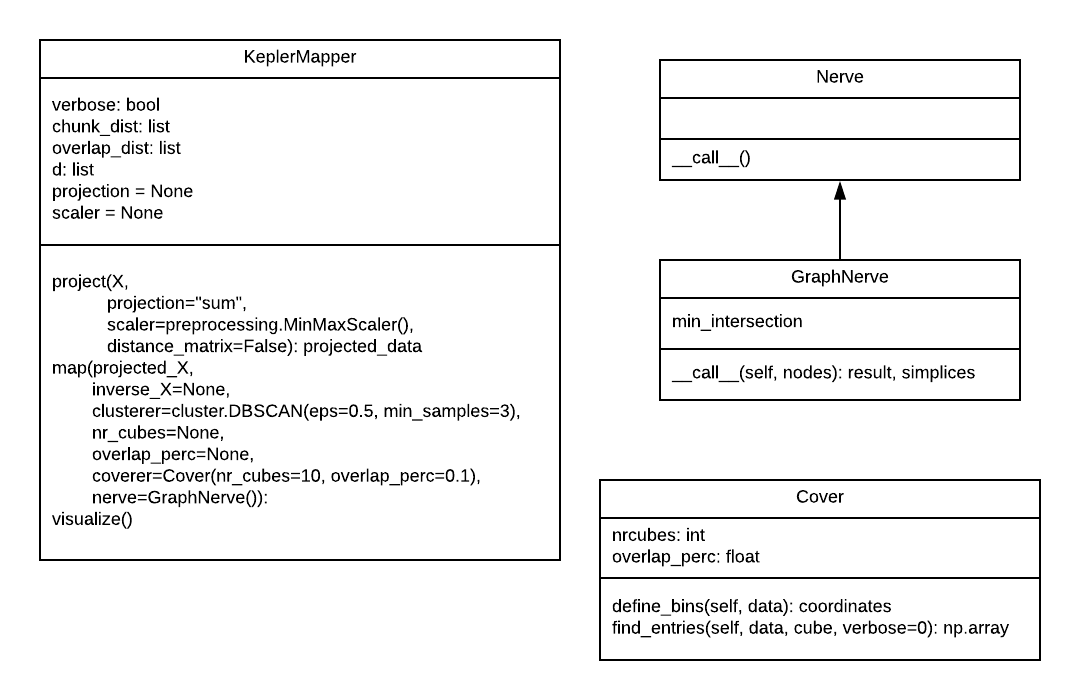
\includegraphics[width=0.8\textwidth]{images/KMapper.png}
\label{fig:keplermapper}
\end{figure}


\subsection{Python Mapper (PyMapper)}
Python Mapper is a Python package developed by Daniel M\"ullner as his PhD thesis. It comes with two companion packages written in C++: $cmappertools$ and $fastcluster$. Compared to Kepler Mapper, it is expected to be:
\begin{itemize}
	\item Comprehensive, thanks to the implementation of more filters, more covers.
	\item Performant, thanks to a custom C++ backend and thus compiled code and efficient multi threading.
	\item Easy to use, thanks to the graphical interface provided.
\end{itemize}

However, this package has the following cons:
\begin{itemize}
\item It is outdated and not maintained any more (Mapper: current release dated April 19, 2017. Cmappertools: current release dated March 2, 2016)
\item The code is not documented. A little documentation is provided for the use of the grapical interface, but there's no documentation about the native Python API.
\item No examples are provided with the code. However, it is possible to see the code generated by the GUI while playing around with simple datasets. An example of code generated by the GUI is given in Listing \ref{list:pymapper}
\item Code's architecture is in my opinion messy and poorly designed: there is no common interface of different filter classes and cover classes. There's a gigantic class $MapperOutput$ that is almost impossible to handle, given the many methods it offers. The code is organized as a mix of object oriented programming and functional programming making it really hard to understand how a modification will affect the whole system. The API of the package is not clear: in other words, it is not clear what is exposed to the user and what should be private.
\item C++ code is really hard to understand, since the original C-Python API is used instead of binding libraries such as PyBind11 (used in lmapper's companion package fastfilter). This makes the binding code really verbose and implementation-dependent.
\item It's really hard to install because of deprecated dependencies.
\item Some C++ implementations of clustering algorithms in $fastcluster$ are now obsolete, since they have been included in more recent releases of SciPy.
\end{itemize}

In figure \ref{fig:pymapper} a simplified UML class diagram of the core code of PyMapper is showed.
\begin{lstlisting}[language=Python, caption=PyMapper example automatically generated from the GUI, label=list:pymapper]
'''
    Python Mapper script
    Generated by the Python Mapper GUI
'''
import mapper
import numpy as np
import matplotlib.pyplot as plt

'''
    Step 1: Input
'''
import gzip
filename = '/Users/martinomilani/Documents/mapper/exampleshapes/cat-reference.csv.gz'
with gzip.open(filename, 'r') as inputfile:
    data = np.loadtxt(inputfile, delimiter=',', dtype=np.float)
# Preprocessing
point_labels = None
mask = None
Gauss_density = mapper.filters.Gauss_density
kNN_distance  = mapper.filters.kNN_distance
crop = mapper.crop
data, point_labels = mapper.mask_data(data, mask, point_labels)
'''
    Step 2: Metric
'''
intrinsic_metric = False
if intrinsic_metric:
    is_vector_data = data.ndim != 1
    if is_vector_data:
        metric = Euclidean
        if metric != 'Euclidean':
            raise ValueError('Not implemented')
    data = mapper.metric.intrinsic_metric(data, k=1, eps=1.0)
is_vector_data = data.ndim != 1
'''
    Step 3: Filter function
'''
if is_vector_data:
    metricpar = {'metric': 'euclidean'}
    f = mapper.filters.eccentricity(data,
        metricpar=metricpar,
        exponent=1.0)
else:
    f = mapper.filters.eccentricity(data,
        exponent=1.0)
# Filter transformation
mask = None
crop = mapper.crop
'''
    Step 4: Mapper parameters
'''
cover = mapper.cover.cube_cover_primitive(intervals=15, overlap=50.0)
cluster = mapper.single_linkage()
if not is_vector_data:
    metricpar = {}
mapper_output = mapper.mapper(data, f,
    cover=cover,
    cluster=cluster,
    point_labels=point_labels,
    cutoff=None,
    metricpar=metricpar)
cutoff = mapper.cutoff.first_gap(gap=0.1)
mapper_output.cutoff(cutoff, f, cover=cover, simple=False)
mapper_output.draw_scale_graph()
plt.savefig('scale_graph.pdf')
\end{lstlisting}

\begin{figure}[h]
\caption{PyMapper Architecture (simplified)}
\centering
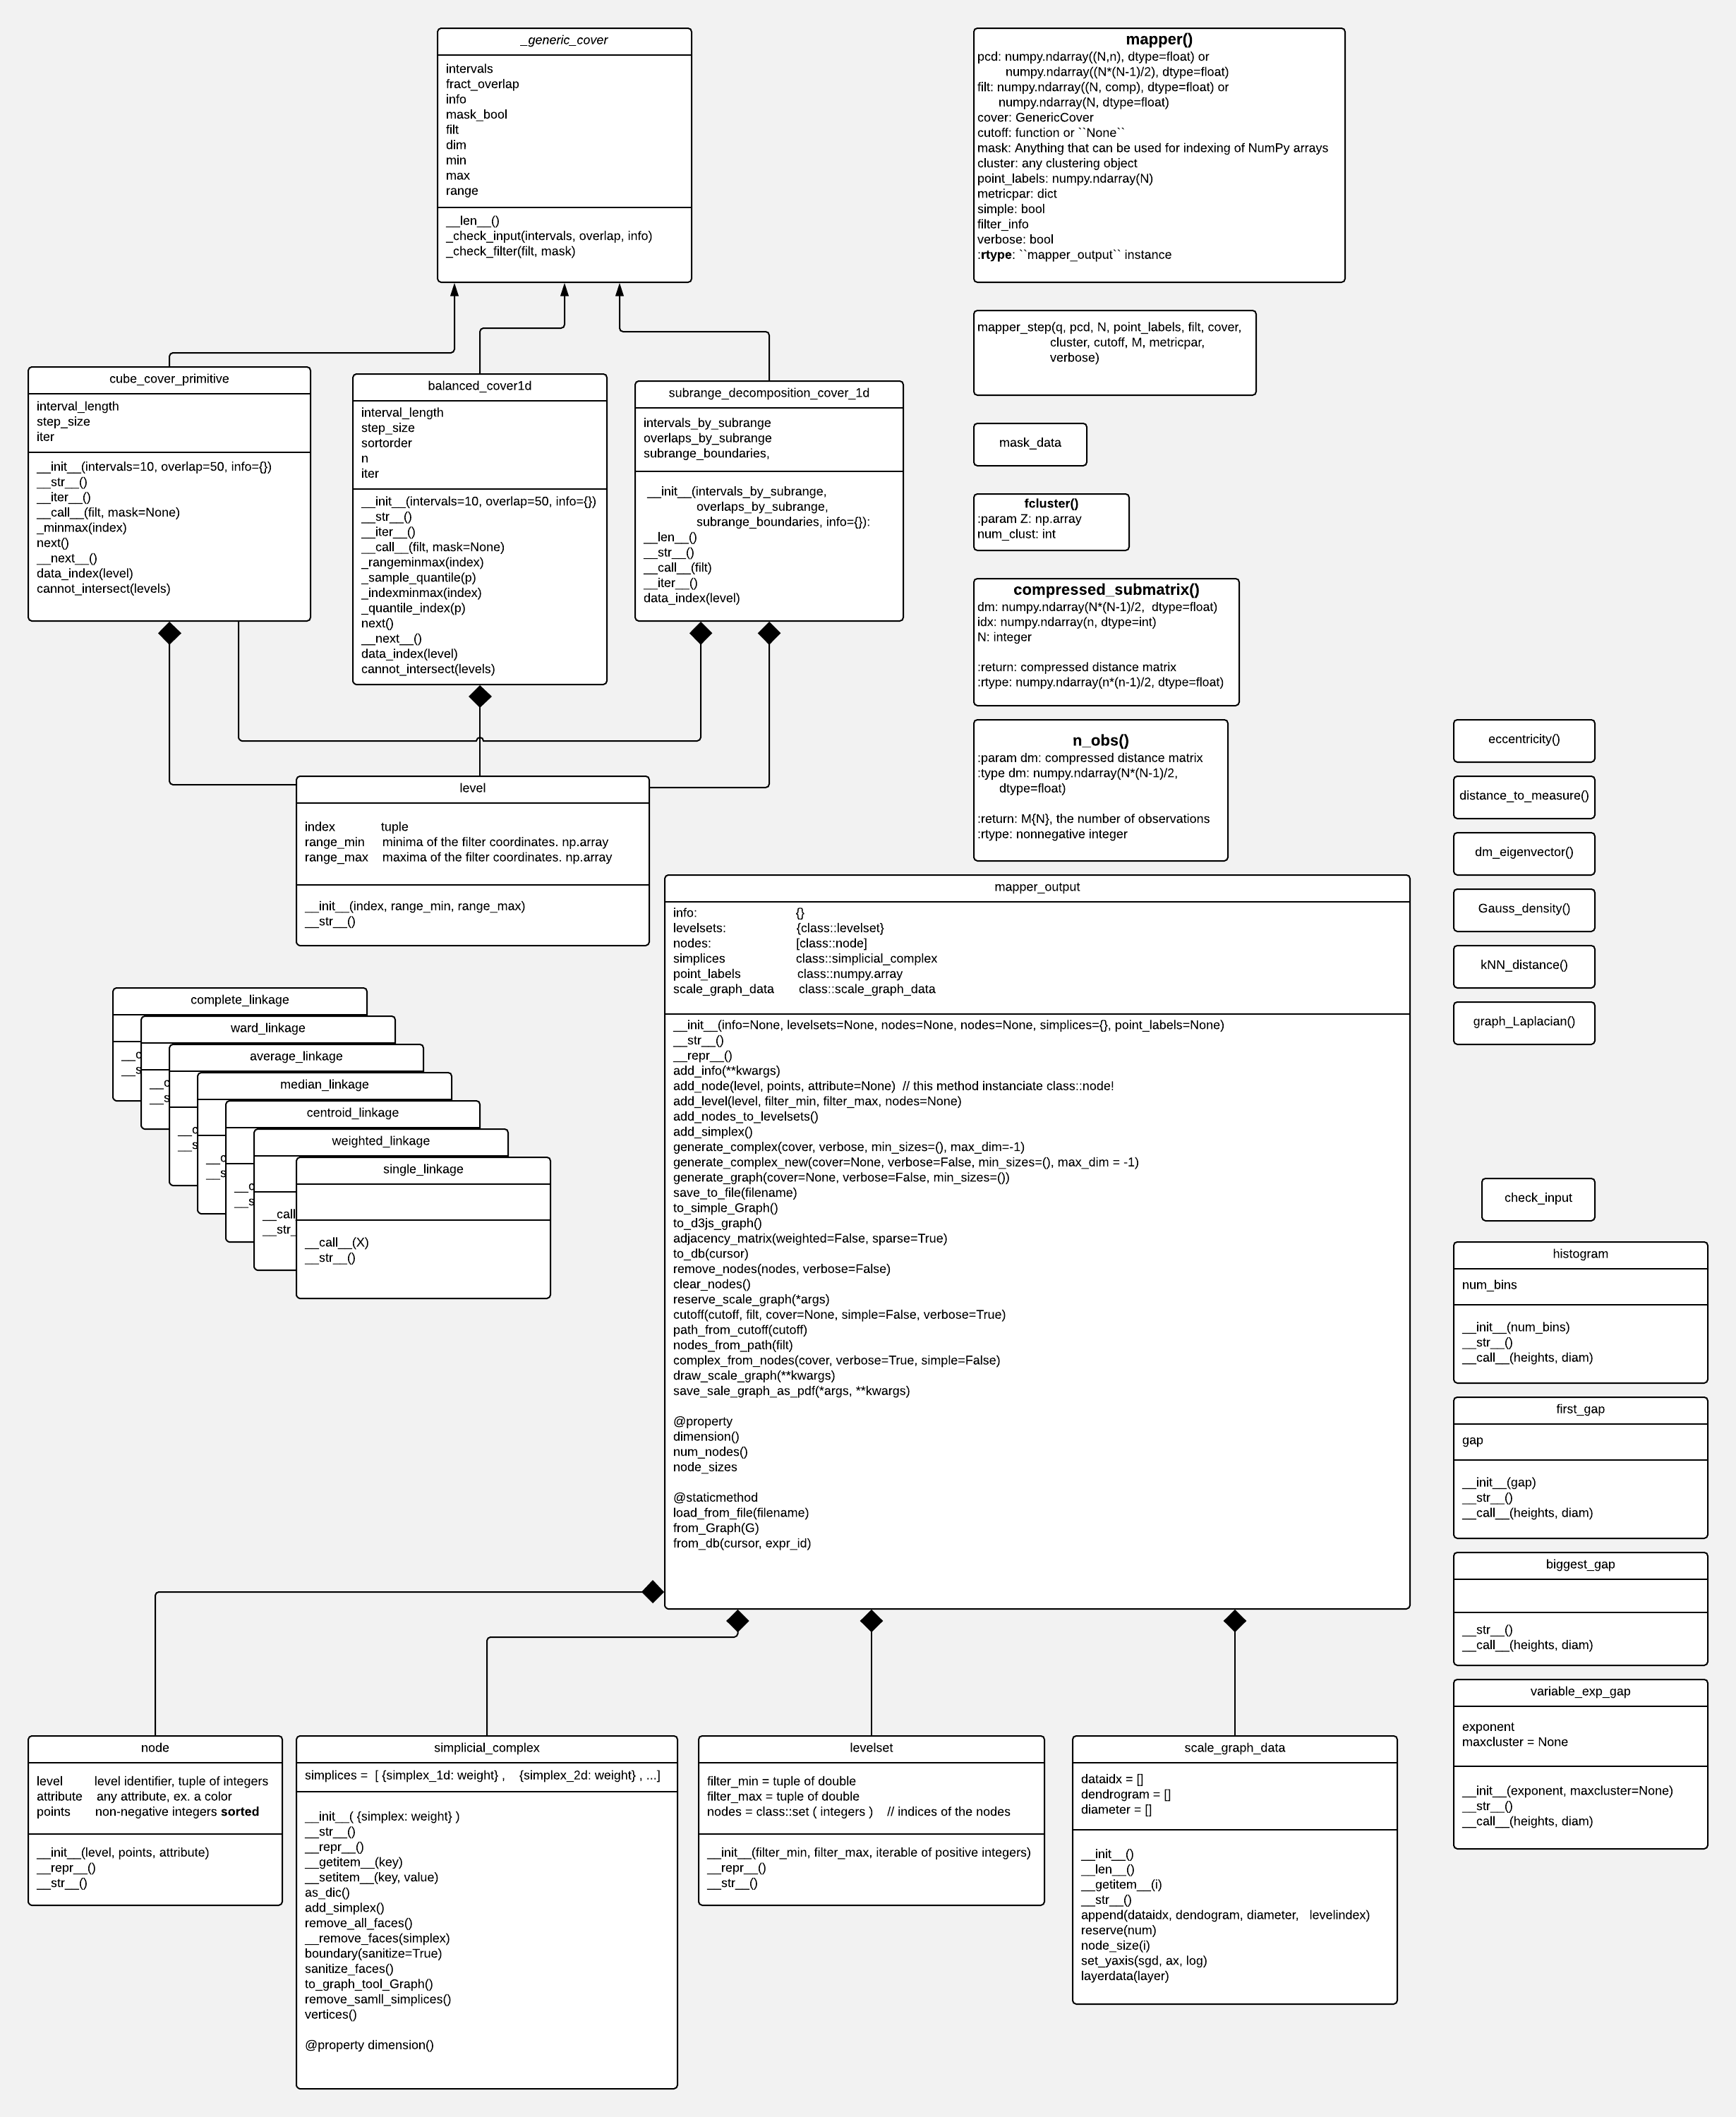
\includegraphics[width=0.8\textwidth]{images/pythonmapper.png}
\label{fig:pymapper}
\end{figure}


\pagebreak

\section{Lmapper}
\subsection{Intro}
The architecture has been inspired to the previous implementation of Daniel M\"ullner \cite{pythonmapper}. Compared to Kepler Mapper, this architecture is complex but more modular. However, the API of such package is too complex to use, and thus we aimed to design a simpler API similar to Kepler Mapper's one.\\
The approach followed for the development of this package was a test-driven approach: first a basic test for the package was written, and then the code necessary to make it work was developed. Once the first test was passed, this procedure was iterated with a more complex test containing more advanced features. This approach was chosen since in this way the development was always guided by a specific goal (pass the test).
We present here under the first two tests that were designed and we comment them.

\paragraph{test 1}
\begin{lstlisting}[language=Python, caption=First test for Mapper]
import lmapper as lm
from lmapper.filter import Projection
from lmapper.cover import UniformCover
from lmapper.cluster import Linkage
from lmapper.cutoff import FirstGap
from lmapper.datasets import circles

def main():
	filter = Projection(ax=0)
	cover = UniformCover(nintervals=15,
										     overlap=0.4)
	cutoff = FirstGap(0.05)
	cluster = Linkage(method='single',
									 metric="euclidean",
									 cutoff=cutoff)
	mapper = lm.Mapper(data=circles,
											filter=filter,
	 										cover=cover,
											cluster=cluster)
	mapper.fit()
	mapper.plot()


if __name__ == "__main__":
main()

\end{lstlisting}
This test shows the main components and design choices of the package. 
\paragraph{Import statements}
The code would be structured in a pure OOP fashion. The package would have been composed by five modules: \_mapper.py, filter.py, cover.py, cluster.py, cutoff.py.  Each module contains the definitions of the classes implementing the corresponding algorithms. 
\paragraph{main()}
First, one object for the filter, one object for the cover, one object for the cutoff method used in the clustering step, one object for the clustering step are instantiated. Given the many parameters of Mapper, in this way each step of the Mapper pipeline is isolated in an object that contains its set of parameters, avoiding long lists of parameters that could make the API confused.\\
These objects (filter, cover, cluster) are then used to instantiate a mapper object together with the data that has to be analyzed. The mapper object has to expose to the client user two methods: fit() and plot().\\
It can be seen that such test looks more readable that the code necessary for PyMapper, but however it let the user set all the parameters that Kepler Mapper hides and does not let the user choose. Plus, the package is clearly modular: if in the future more algorithms would be necessary (i.e. a new way of building a cover, or a new clustering algorithm) it would be necessary to implement a corresponding new class respecting the API of the backend to correctly interact with the other modules, expose it to the user and all the future patches of the package would make all the old client code still compatible.\\

\paragraph{test 2}
\begin{lstlisting}[language=Python, caption=Second test for Mapper]
import lmapper as lm
from lmapper.filter import Projection
from lmapper.cover import UniformCover
from lmapper.cluster import Linkage
from lmapper.cutoff import FirstGap
from lmapper.datasets import circles

def main():
	filter = Projection(ax=0)
	cover = UniformCover(nintervals=15,
											 overlap=0.4)
	cutoff = FirstGap(0.05)
 	cluster = Linkage(method='single',
									 metric="euclidean",
									 cutoff=cutoff)
	mapper = mp.Mapper(data=circles,
											 filter=filter,
											 cover=cover,
											 cluster=cluster)
	mapper.fit()
	mapper.plot()
	
	cluster = Linkage(method='average',
									 metric='correlation',
									 cutoff=cutoff)
	mapper.set_params(cluster=cluster)
	mapper.fit()
	mapper.plot


if __name__ == "__main__":
main()

\end{lstlisting}
This test was designed to solve the following issue: Mapper has a lot of parameters, and to set them correctly a lot of trial-and-error has to be done by the user to find a good choice of parameters. All the previous implementations taken in exam in this work, when a parameter is changed, need to recalculate everything from scratch, making the trial-and-error procedure really slow and annoying. However, Mapper is an algorithm that has a clear pipeline
\begin{enumerate}
	\item Calculate the filter values
	\item Calculate the pull-back cover
	\item Cluster each element of the pullback cover
	\item Build the simplicial complex from the elements of the pullback cover
\end{enumerate}
Each one of these steps is completely independent from the previous ones; this means that if we fit a Mapper object, and then we decide to try to fit it with a change of the clustering method, there's no need to recompute the filter values and the pullback cover, and the computations could restart from step (3). To enable this we need to design the Mapper class to store all the intermediate information needed to restart the computation from whichever step, and make it "aware" of the changes to the previous set of parameters through the method set\_params().\\
We want to underline that this design represents a completely new feature that was never implemented before in our knowledge.\\
\paragraph{Base architecture}
In figure \ref{fig:basearchitecture} the architecture for a first implementation of the package necessary to pass the first two tests is illustrated. The final version of the package is more complex, but this is sufficient to illustrate the high level design choices that were respected during the whole development. The real architecture will be discussed in details later on.\\
\begin{figure}[h]
	\caption{Simplified Mapper Architecture (simplified)}
	\centering
	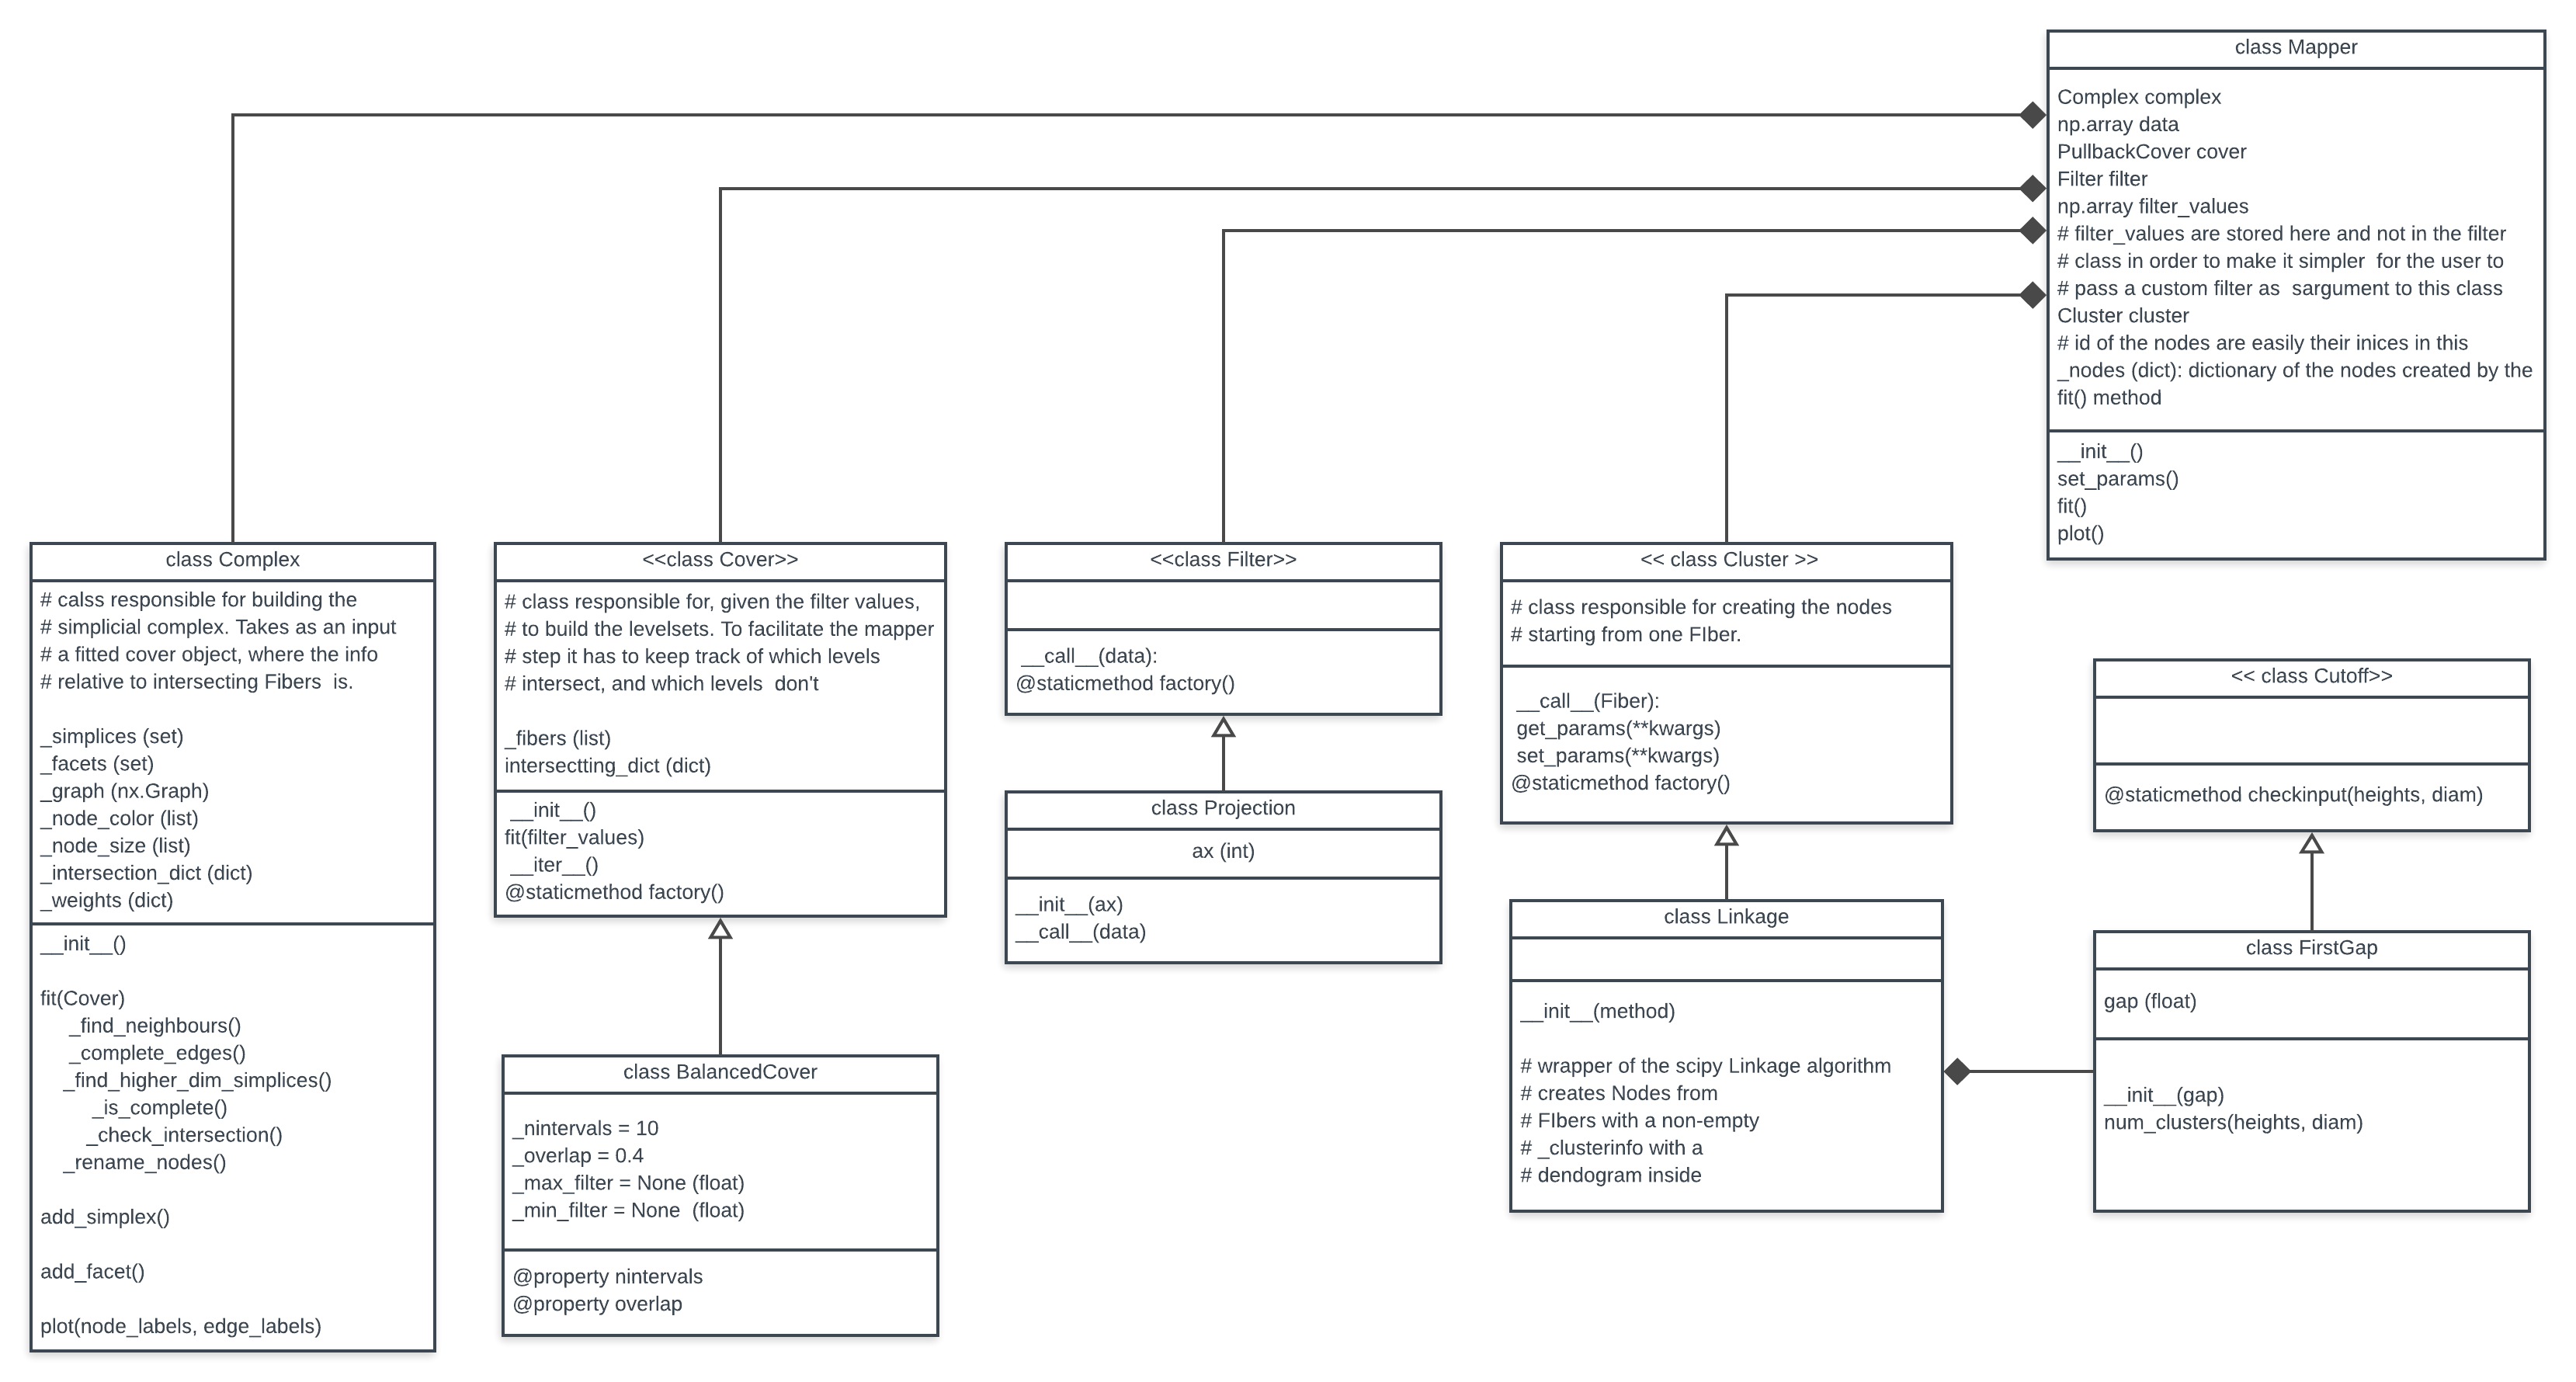
\includegraphics[width=1\textwidth]{Figs/SimplifiedArchitecture.png}
	\label{fig:basearchitecture}
\end{figure}
Three classes \textit{class Filter, class Cover, class Cluster} defining the API of the backend of the package are defined, one for each of the first three steps of the Mapper pipeline. Every class implementing an algorithm for a pipeline step has to derive from one of these classes,  in order to be compatible with the package. \textit{class Complex} is responsible for the fourth and last step of the Mapper pipeline. The classes exposed to the user would be only \textit{class Mapper, class Projection, class BalancedCover, class Linkage}. All the other classes, explained in detail later on, will be part of the backend of the package, and thus should not be used in any client code.

\subsection{Description of the classes}
In figure \ref{fig:fullmapperarchitecture} we present the UML graph of the final version of the package.
\begin{figure}[h]
	\caption{Full Mapper Architecture}
	\centering
	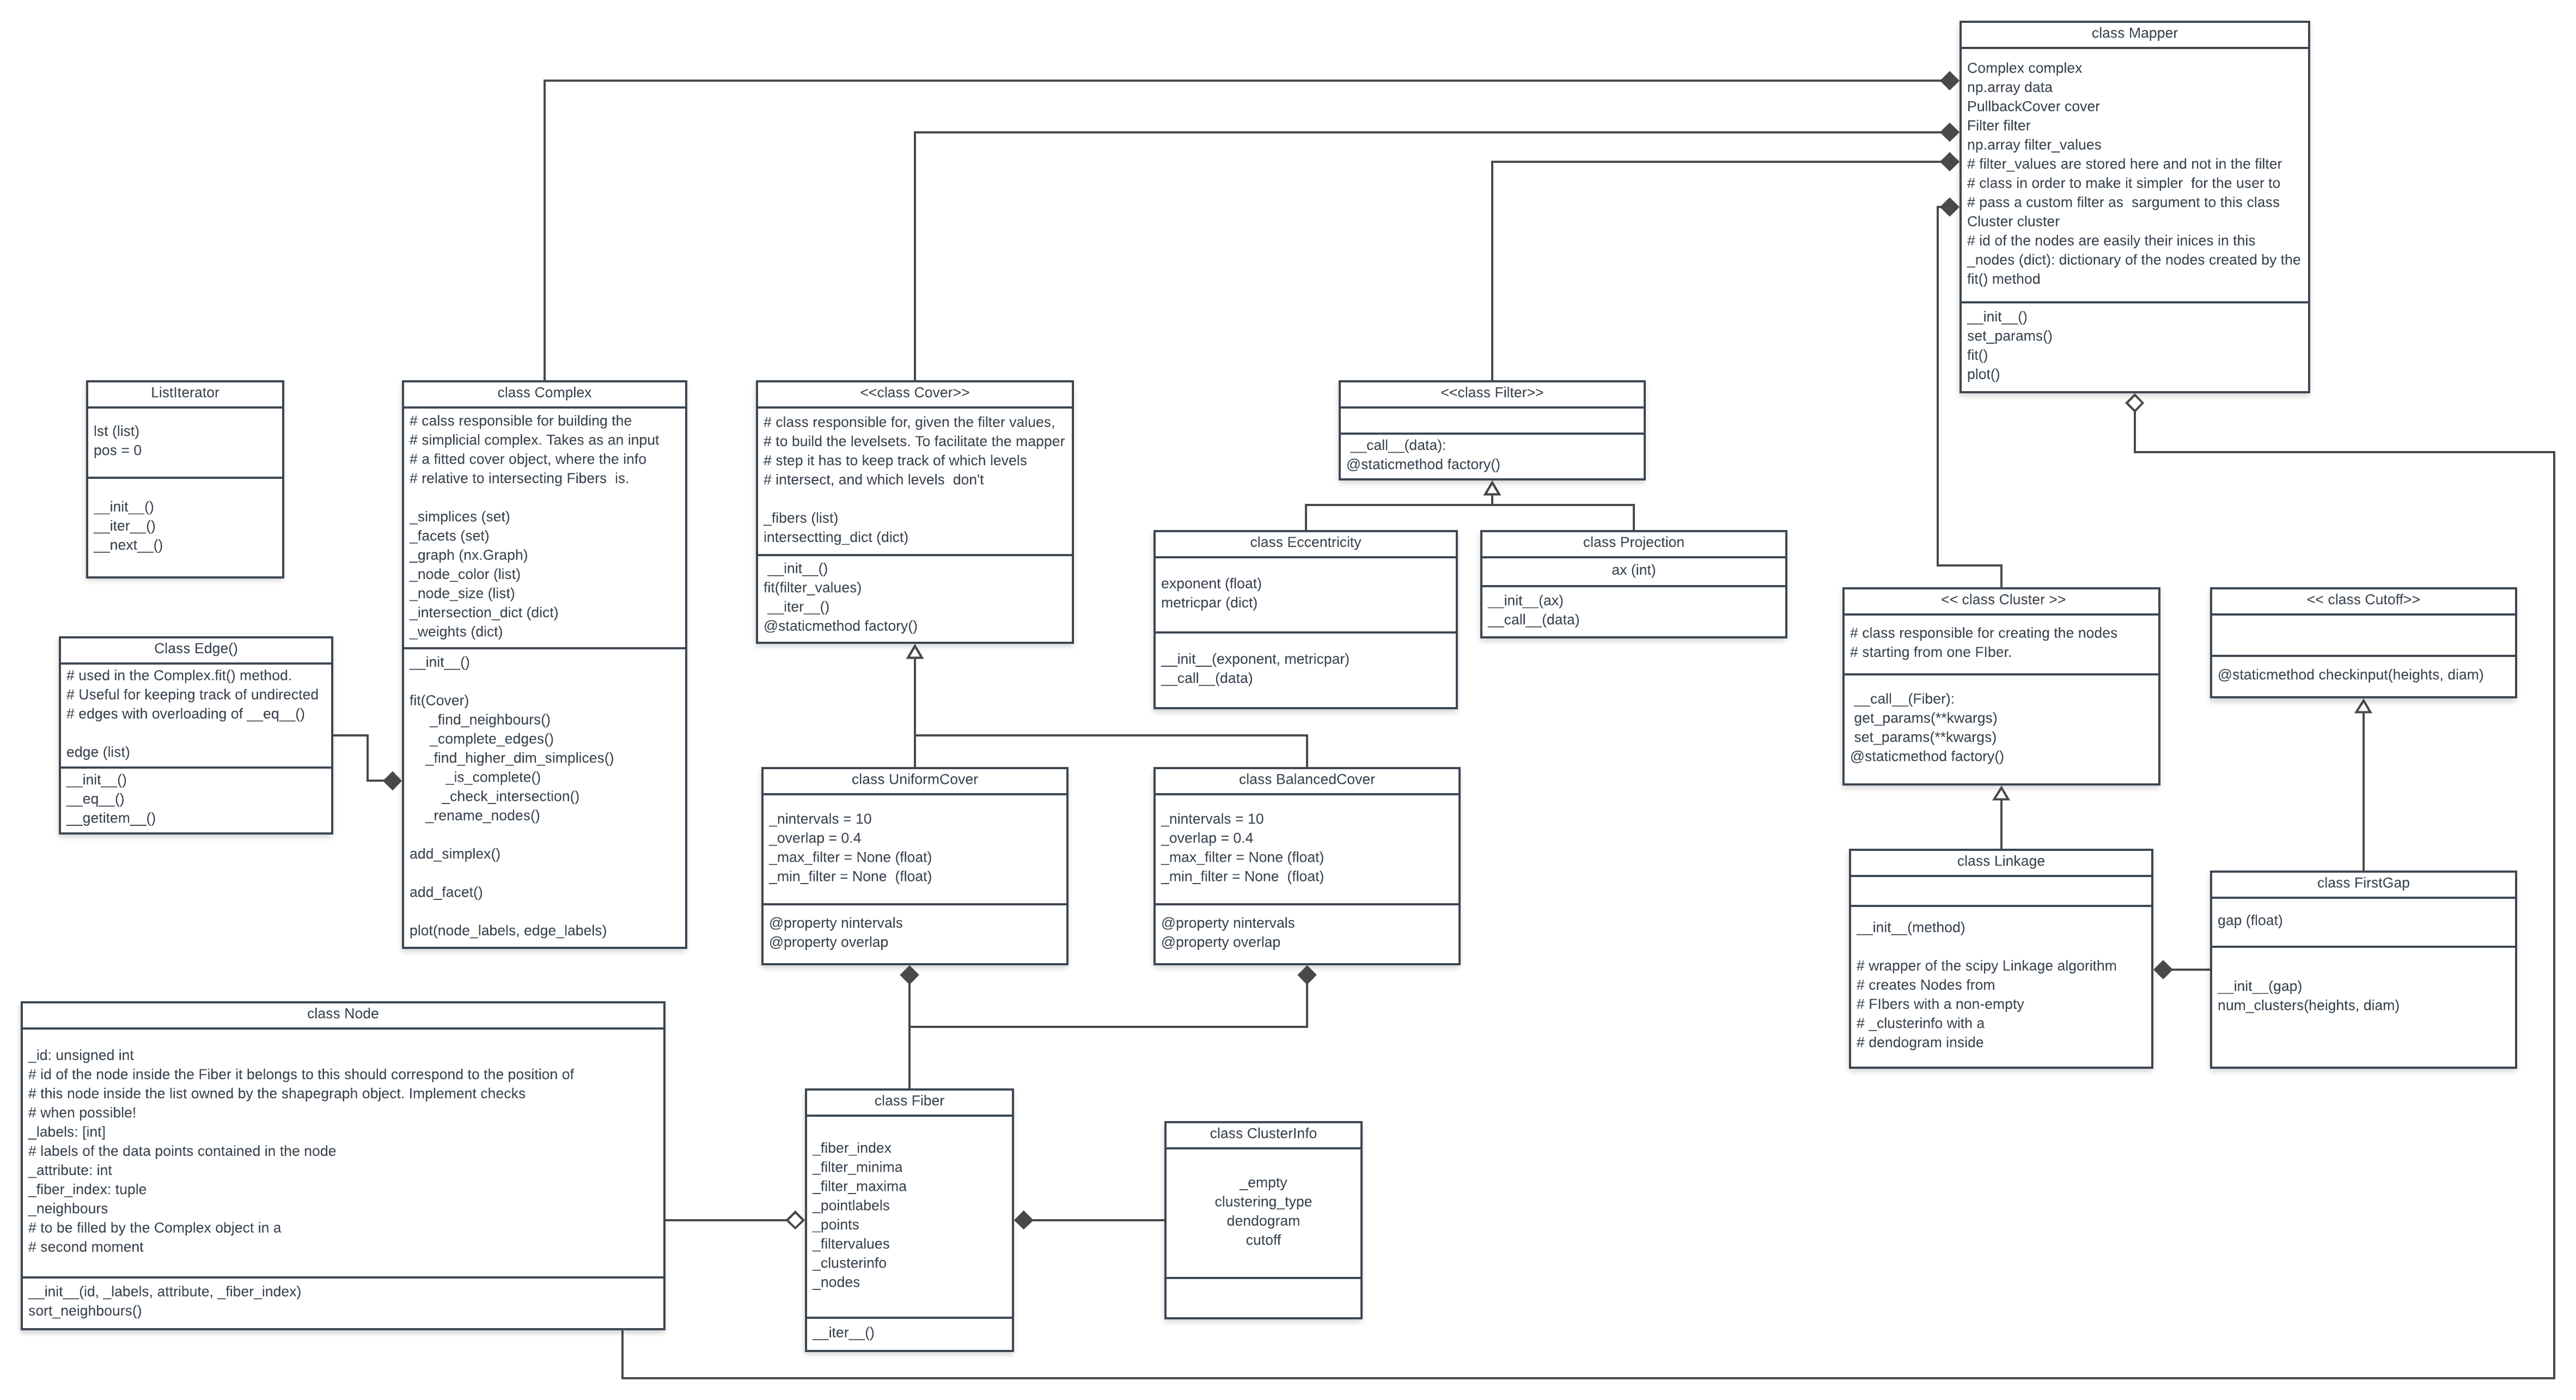
\includegraphics[width=1\textwidth]{Figs/fullMapperArchitecture.png}
	\label{fig:fullmapperarchitecture}
\end{figure} 
In this section we present the classes in a top-to-bottom order in order to first present the classes implementing the most high level algorithms, and only at the end present the classes implementing the low level details.

\subsubsection{\textit{class Mapper}}
\begin{lstlisting}[language=Python, caption=Example for the Mapper class]
import lmapper as lm
from lmapper.filter import Projection
from lmapper.cover import UniformCover
from lmapper.cluster import Linkage
from lmapper.cutoff import FirstGap
from lmapper.datasets import circles

filter = Projection(ax=0)
cover = UniformCover(nintervals=15,
                   overlap=0.4)
cluster = Linkage(method='single',
                 cutoff=FirstGap(0.05)
mapper = lm.Mapper(data=circles,
                   filter=filter,
                   cover=cover,
                   cluster=cluster)
mapper.fit()
mapper.plot()
\end{lstlisting}

\begin{lstlisting}[language=Python, caption=Example 2 for the Mapper class. The Mapper object can be initialized just with the data matrix.]
import lmapper as lm
from lm.datasets import circles

mapper = lm.Mapper(data=circles)
mapper.fit()
mapper.plot()
\end{lstlisting}

\begin{lstlisting}[language=Python, caption=Example 3 for the Mapper class. The arguments of the init function can be strings.]
import lmapper as lm
from lm.datasets import circles

mapper = lm.Mapper(data=circles,
										filter='Projection',
										cover='UniformCover',
										cluster='Linkage')
mapper.fit()
mapper.plot()
\end{lstlisting}

\begin{lstlisting}[language=Python, caption=Example 4 for the Mapper class. The filter given to the init function of the Mapper object can be a Python function.]
import lmapper as lm
from lmapper.cover import UniformCover
from lmapper.cluster import Linkage
from lmapper.cutoff import FirstGap
from lmapper.datasets import circles

def ProjectionOnFirstCoordinate(x):
	return x[:, 0]
	
cover = UniformCover(nintervals=15,
										 overlap=0.4)
cluster = Linkage(method='single',
								 cutoff=FirstGap(0.05)

mapper = lm.Mapper(data=circles,
										filter=ProjectionOnFirstCoordinate)
mapper.fit()
mapper.plot()
\end{lstlisting}


As shown in the example he Mapper init method requires four arguments: the data matrix as a two-dimensional numpy array, where the $n-th$ row represents the coordinates of the $n-th$ data point; the filter object, the cover object, and the cluster object. //
We present now the main original features of this implementation of the Mapper algorithm, that haven't been implemented neither in Kepler Mapper neither in Python Mapper.

\paragraph{Optimized calls to fit()}
The main feature of this implementation is that it is optimized for minimizing the computational time required for multiple calls to the fit() method. Since there's no way of algorithmically test the goodness of a Mapper parameters set, the only way to find a good combination of parameters is to manually explore the parameter space and observing the corresponding output graph. This is illustrated in the following example.

\begin{lstlisting}[style=mystyle, deletekeywords={filter}]
import lmapper as lm
from lmapper.filter import Projection
from lmapper.cover import UniformCover
from lmapper.cluster import Linkage
from lmapper.cutoff import FirstGap
from lmapper.datasets import circles

filter = Projection(ax=0)
cover = UniformCover(nintervals=15,
								   overlap=0.4)
cluster = Linkage(method='single',
						   cutoff=FirstGap(0.05)

mapper = lm.Mapper(data=circles,
								 filter=filter,
								 cover=cover,
								 custer=cluster)
mapper.fit()
mapper.plot()

# we want to see what happens if we change the clustering step
# from a Single Linkage to an Average Linkage,
# mantaining all the rest of the Mapper parameters equal. 
# For this purpose we use the set_params() method

mapper.set_params(cluster= Linkage(method='average', cutoff=FirstGap(0.05))

# After having changed the parameters, we need to fit the Mapper object
mapper.fit()

# Now we can plot the new mapper graph to compare it with the previous one
mapper.plot()
\end{lstlisting}

Since in practice it is normal to alternate many calls to fit() and set\_params() to find a good parameter set, the fit() method has been implemented in order to avoid to alway recompute everything from scratch. The Mapper algorithm has indeed a clear pipeline presented in section 2.1. If as in the example above we change only the parameters of the clustering step, it is useless to recompute the filter values and the cover, already calculated before. For this reason, the Mapper class keeps track internally of its state, what has changed compared to the previous state, and the new call to the fit() method performs only the computations needed. In the example, only the clustering step will we done before computing the output graph.
\subsubsection{\textit{class filter.Filter}} \label{subsubsection:class filter.Filter}
Python do not provide the opportunity of defining abstract classes. However, given the non trivial complexity of the package, we chose to the define anyway a base class for each step of of the Mapper pipeline to provide a clear way of understanding the interface of the backend API. \textit{Each one of these four classes} \lstinline{class filter.Filter, class cover.Cover, class cluster.Cluster, class cutoff.Cutoff} \textit{was written in order that every time a new filter, cover, cluster, cutoff has to be implemented, it will be implemented as a class derived from one of these corresponding base classes}. For example, a projection filter has to be implemented as child class of the corresponding Filter class: \lstinline|class Projection(Filter)|. For example, the programmer that will be expanding the package by adding a new filter, will have to read the code of the Filter class to see which methods have to be overridden, and which methods are already provided in the base class. In this way these four base classes act as a guideline for the programmer to make sure that every newly added class will respect the backend API of the package.\\The class Filter simply declares the \lstinline{__call__()} operator raising a \lstinline{NotImplementedError} exception, indicating to the programmer that any new filter has to override such a method. Since Python is not type-checked (although the package \textbf{typing} could be used from Python 3.5) it was chosen to put clear indications of the expected parameter and the return value type In the docstring of the \lstinline{filter.Filter.__call__()} method. The same procedure has been used for all the methods of the thee other base classes \lstinline{class filter.Filter, class cover.Cover, class cluster.Cluster, class cutoff.Cutoff} raising a \lstinline{NotImplementedError} exception.\\ A static factory method necessary for the instantiation of the Filter object when the Mapper object is instantiated with only strings as arguments. Note that the code of \lstinline{filter.Filter.factory()} does not have to be updated every time a new child class is added to the package thanks to the use of the \lstinline{globals()} method.

\subsubsection{\textit{class filter.Eccentricity(filter.Filter)}}
This implements the eccentricity filter as presented in \cite{pythonmapper}. In short, the eccentricity filter value of the $n-th$ data point is the p-norm of the $n-th$ row of the distance matrix
$$Eccentricity(x_i; p) = \left(\sum_{k=0}^{N} d(x_i, x_k)^p\right)^\frac{1}{p}$$
As explained above in section \ref{subsubsection:class filter.Filter} we can see that this class is a child of \lstinline|filter.Filter|. It implements an \lstinline|__init__()| method initializing the attributes that every cover object must have and overrides the method \lstinline|__call__()| as indicated in the docstring of the same method of the base class \lstinline|filter.Filter.__call__()|.\\
Since the computation of the eccentricity is computationally very expensive because of the calculation of the full distance matrix, the implementation of the Python functions \lstinline{eccentricity()} and \lstinline{my_distance()} were implemented in C++ and are available in the module \textbf{filterutils}. They provide an efficient parallel implementation of the most CPU-intensive part of the algorithm through the use of OpenMP.\\
When the package \textbf{lmapper} is imported, the module \textbf{filterutils} is imported. If the latter import fails, the user is notified about the failure with a printed message on the terminal and a slower, fully Python implementation of the functions \lstinline{eccentricity()} and \lstinline{my_distance()} provided in the \textbf{filter.py} module is used instead.\\
A last method, \lstinline|filter.Eccentricity.for_assignment_only()| is defined. However, this method is meant to be used from the companion package \textbf{predmap} and not to be exposed to the final user of the package. This implementation is however not clean and prone to bugs, since it makes the implementations of the two packages profoundly interdependent. This method is necessary as the \lstinline|filter.Filter.__call__()| method is meant to operate on two-dimensional \lstinline|np.ndarray| representing the whole data matrix in order to vectorize as much as possible the computations to achieve speedup. However, we'll see that in \textbf{predmap} it is necessary to compute the filter values \textit{of only one new data point belonging to the test set after having already computed the filter values of the whole original data matrix of the training set}. These two different situations of calculating filter values require two different implementations. It is not clear if the implementation needed in the second scenario was to be implemented in \textbf{predmap} or in \textbf{lmapper}. For now it has been chosen to add this method \lstinline|filter.Eccentricity.for_assignment_only()|. A more elegant solution is left as further work.

\subsubsection{\textit{class cover.Cover}}
As explained above in section \ref{subsubsection:class filter.Filter} \lstinline|class cover.Cover| is a base class to define the common interface that any new implementation of a new cover method must respect. Similar to \lstinline|filter.Filter| it implements an \lstinline|__init__()| method initializing the attributes that every cover object must have. It implements a method \lstinline{cover.Cover.find_intersecting_dict()} that outputs a dictionary that keeps track of which fibers intersect. This implementation is valid as soon as the filter values are one dimensional, and each Fiber object represents is the counter image of an interval on the real line. When the package will be expanded with multi-dimensional filters, or with more complicated ways of building a cover, this method will become obsolete and must be changed.
\subsubsection{\textit{class cover.UniformCover(OverlapCover)}}
It derives from \lstinline|class OverlapCover(Cover)|. This latter class was introduced since \lstinline|class UniformCover(OverlapCover), KeplerCover(OverlapCover), BalancedCover(OverlapCover)| share the common idea of being defined by overlapping intervals on the image of the filter $f(X)\subset\mathcal R$. We can see that  \lstinline|class cover.UniformCover(OverlapCover)| just needs to define the \lstinline{cover.UniformCover.fit()} method, in which the particular construction of this specific cover is implemented. Note that "constructing a cover" for an \lstinline{OverlapCover} means finding the variables  \lstinline|list_of_as| and  \lstinline|list_of_bs| that are respectively the list of the leftmost extremes and the rightmost extremes of the intervals $I_j=(a_j, b_j)$ forming the open cover $\mathcal I = \{I_j\}$ of $f(X)$. Once defined these intervals, all the rest of the implementation is taken care of by the method \lstinline|cover.OverlapCover.find_entries()| that finds the corresponding data points belonging to each preimage $f^{-1}(I_j)$ and instantiating an object of class \lstinline|cover.Fiber| for each preimage $f^{-1}(I_j)$. The output  of \lstinline|cover.OverlapCover.find_entries()| is a list of \lstinline|cover.Fiber| objects, and a dictionary created by the \lstinline|cover.Cover.find_intersecting_dict()| method.
\subsubsection{\textit{class cover.Fiber}}
\lstinline|class cover.Fiber| is just a data structure containing informations relative to each preimage $B_i$ of the pullback cover $\mathcal B = \{B_i\}$. It stores the indices of the data points that the corresponding preimage $B_i$ contains, their filter values, and other useful information.
\subsubsection{\textit{class complex.Node}}
Class responsible for storing the information of one node of the final complex, result of the cluster call on a Fiber. The objects of class Node are stored (owned) by objects of class Fiber and instantiated by the \_\_call\_\_()method of an object of class cluster.Cluster.
\subsubsection{\textit{class ClusterInfo}}
Data structure containing information about the parameters of the clustering algorithm used to produce the Nodes. Objects of class ClusterInfo are owned by Fiber objects. 
\subsubsection{\textit{class cluster.Cluster}}
Abstract class implementing the interface for any Cluster Object.
\subsubsection{\textit{class cluster.Linkage}}
Example of Cluster object. The \_\_cal\_\_() method takes a Fiber, accesses to its data points and cluster them. Each cluster is represented by one Node object, that is owned by the corresponding fiber in its list attribute Fiber.\_nodes.
\subsubsection{\textit{class cutoff.Cutoff}}
The Cutoff class is an abstract class providing the interface for each different cutoff object
\subsubsection{\textit{class cutoff.FirstGap}}
Example of Cutoff. This class implements the First Gap method illustrated by Carlsson et al. in \cite{PAD}. It is used by the cluster.Linkage class to determine the number of clusters to create starting from the full linkage matrix.
\subsubsection{\textit{class complex.Complex}}
Class responsible for storing all the simplices, edges, nodes of the Nerve Complex output of the Mapper algorithm. It also implements a method for drawing te 1-skeleton of the nerve complex. Starting from a Cover object the fit() method accesses all the fibers, all the corresponding nodes and looks for intersections between nodes, creating a corresponding Nerve Complex stored as a list of simplices in the \_simplices attribute. The corresponding 1-d skeleton is stored in the NetworkX.Graph attribute complex.Complex.\_graph. 


\pagebreak

\section{PredMap}
\subsection{Intro}
\subsection{Description of the Classes}
\pagebreak

\section{Fastfilter}
\subsection{Intro}
\pagebreak

%!TEX root = 0.main.tex
\section{Benchmark}

\subsection{lmapper VS kmapper}
We benchmarked lmapper against Kepler Mapper. To benchmark it a specific cover was implemented in \lstinline|lmapper.cover.KeplerCover| in order to implement the same method to build the cover. In both cases the filter used is a projection, since Kepler Mapper do not implement the Eccentricity filter. For this reason it is not possible to take advantage of the \lstinline|filterutils| package. As a clustering algorithm it was used a single linkage algorithm, where for lmapper the \lstinline|cutoff.FirstGap| class has been used to find the number of clusters, whereas for kmapper it was only possible to set a predetermined number of clusters, that has been chosen to be 2. Note that the performances of \lstinline|lmapper| are highly dependent on the parameter chosen to initialize \lstinline|cutoff.FirstGap|. Specifically, the smaller the parameter, the more clusters will be created and the slower will be the method \lstinline|complex.Complex.fit| affecting the overall performances of the package. For this benchmark this parameter has been set in order to obtain a graph the most similar to the one obtained by Kepler Mapper.

\textbf{Hardware used}:
Mac Book Pro late 2011 13", with a 32 nm "Sandy Bridge" 2.4 GHz Intel "Core i5" processor (2435M), 8 GB of 1333 MHz DDR3 SDRAM in two modules of 4GB each.

\begin{figure}[h]
	\caption{Synthetic dataset: performance comparison}
	\centering
	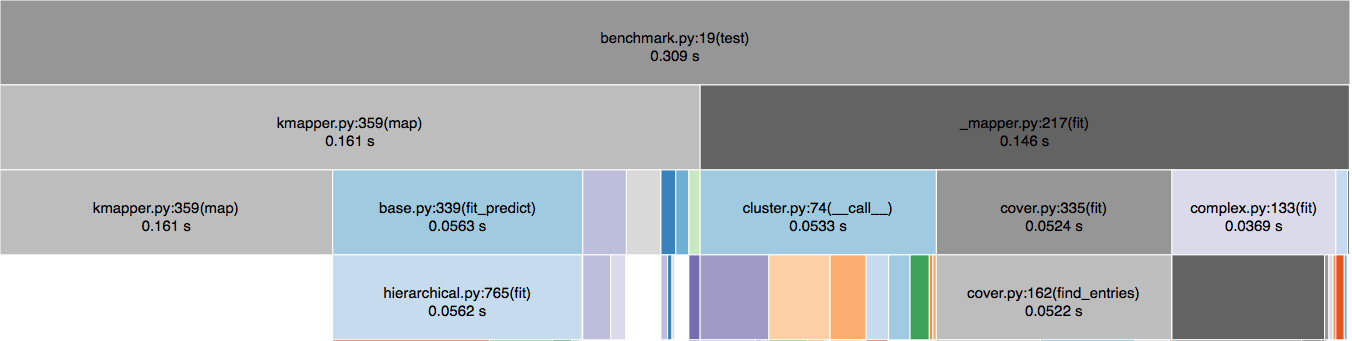
\includegraphics[width=0.9\textwidth]{images/benchmark/synthetic/benchmark}
\end{figure}
\begin{figure}[h!]
	\caption{Synthetic dataset: Left: graph obtained with Kepler Mapper. Right: graph obtained with lmapper}
	\centering
	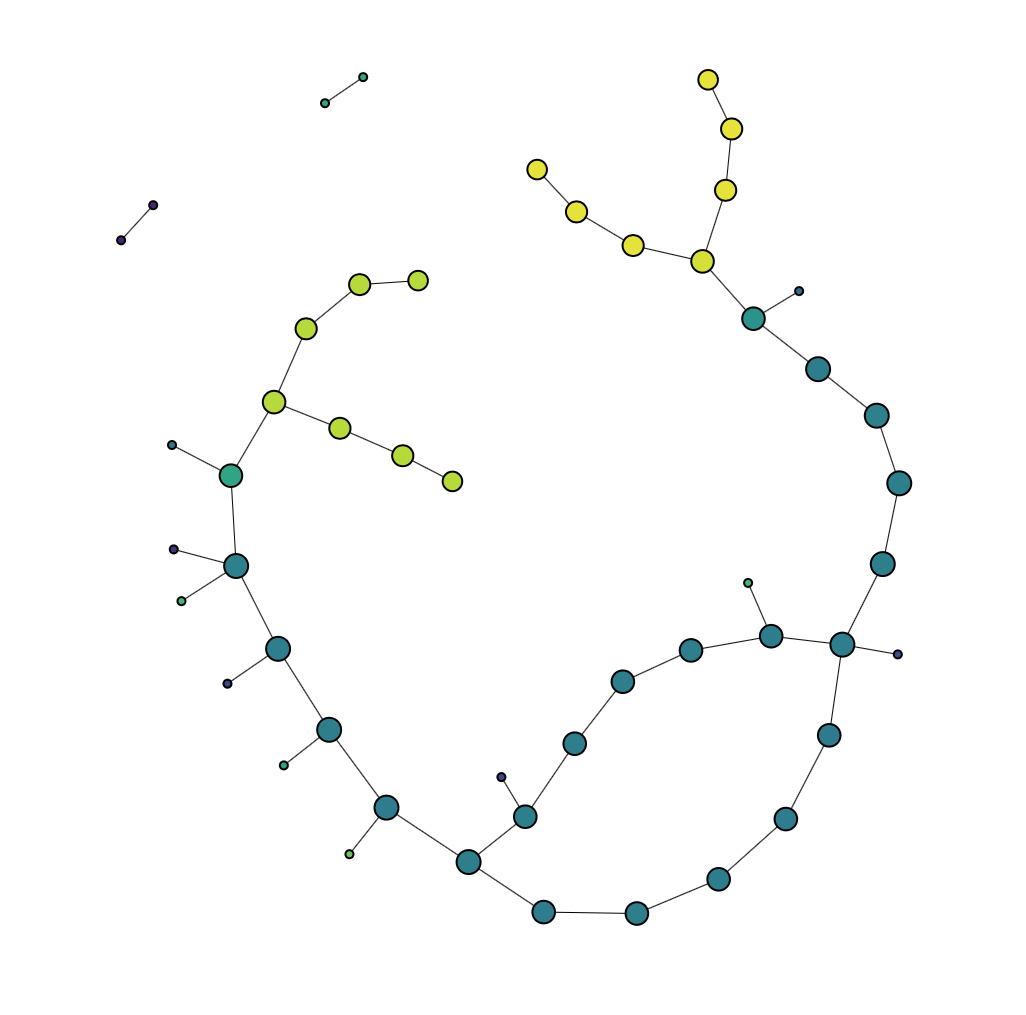
\includegraphics[width=0.4\textwidth]{images/benchmark/synthetic/benchmark_kmapper}
	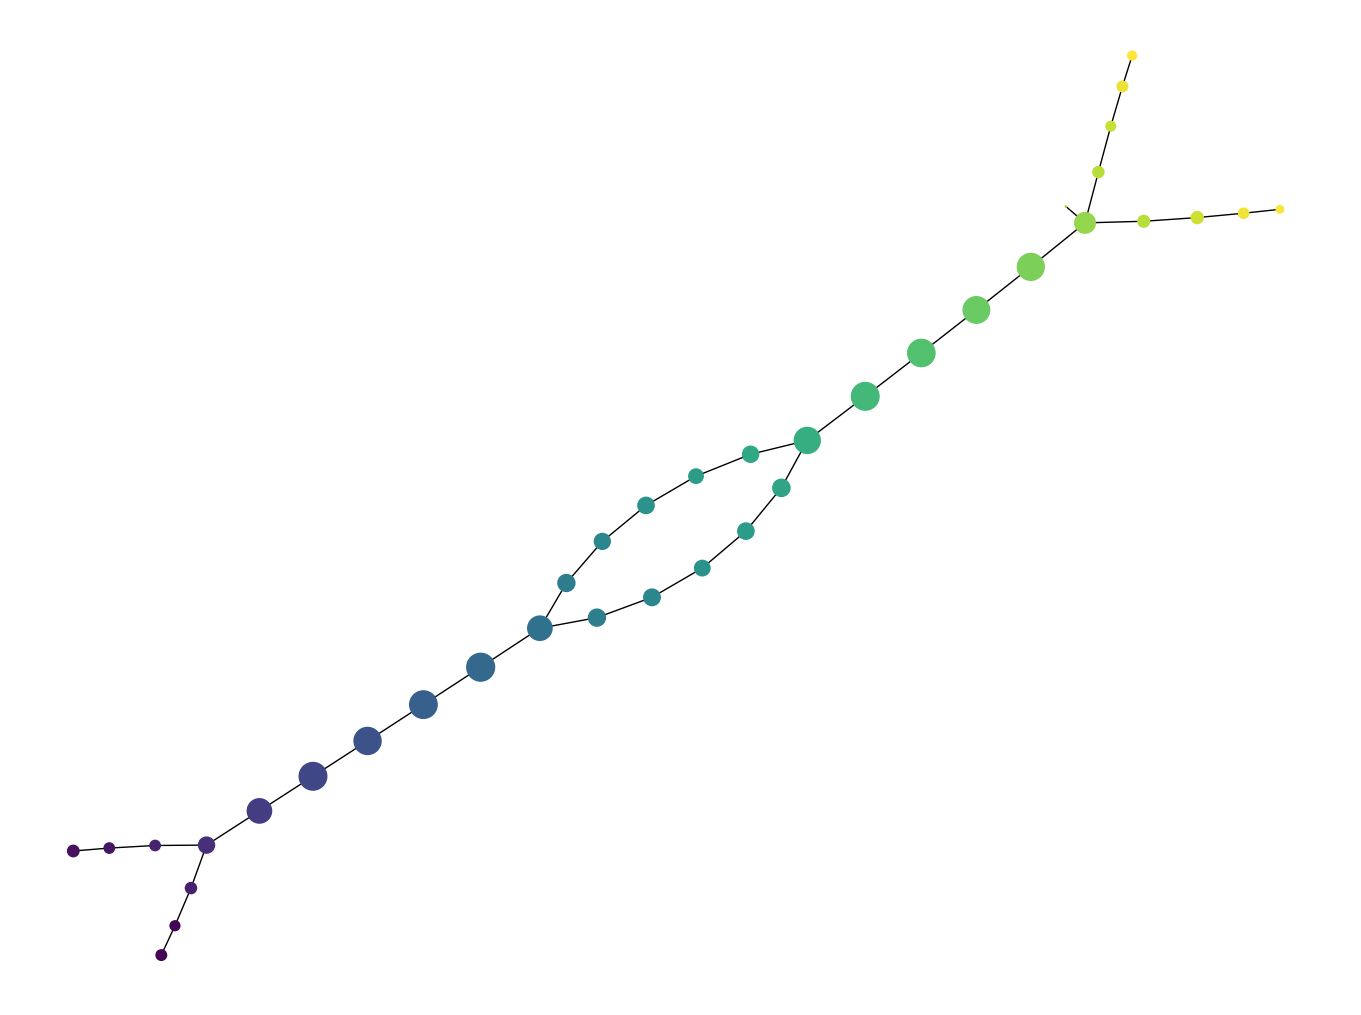
\includegraphics[width=0.4\textwidth]{images/benchmark/synthetic/benchmark_lmapper}
\end{figure}


On the synthetic dataset lmapper managed to get approximately a 10\% speedup compared to kmapper. The main topological features (the four branches and the ring at the center of the data point cloud) are correctly identified by both packages; furthermore we can see how the graph output of lmapper has much less noise than the graph obtained by kmapper. In the graph output of kmapper there are two small extra connected components, plus there are many little nodes connected to the biggest connected component. This was possible thanks to the class lmapper.cutoff.FirstGap that for each set of the cover calculates the number of clusters (nodes) to create from the dendrogram; in kmapper the number of clusters has to be fixed; in this case it was set to 2. This is what causes the creation of many little nodes (noise) in the kmapper output.

In conclusion, lmapper is faster and more robust to noise.

\begin{figure}[h]
	\caption{Wisconsin breast cancer dataset: performance comparison}
	\centering
	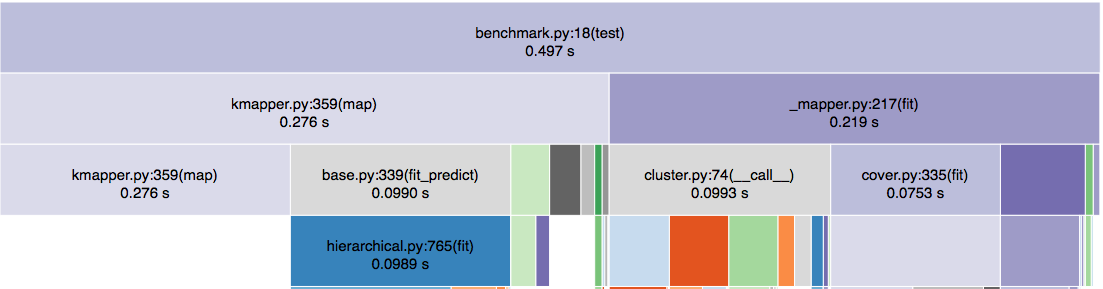
\includegraphics[width=0.9\textwidth]{images/benchmark/cat/benchmark}
\end{figure}
\begin{figure}[h!]
	\caption{Wisconsin breast cancer dataset. Left: graph obtained with Kepler Mapper. Right: graph obtained with lmapper}
	\centering
	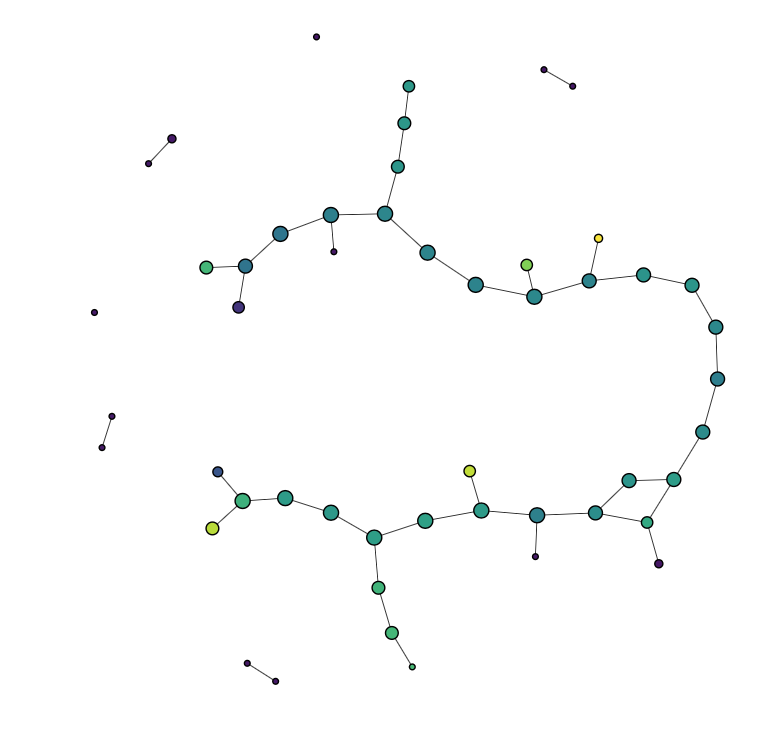
\includegraphics[width=0.4\textwidth]{images/benchmark/cat/benchmark_kmapper}	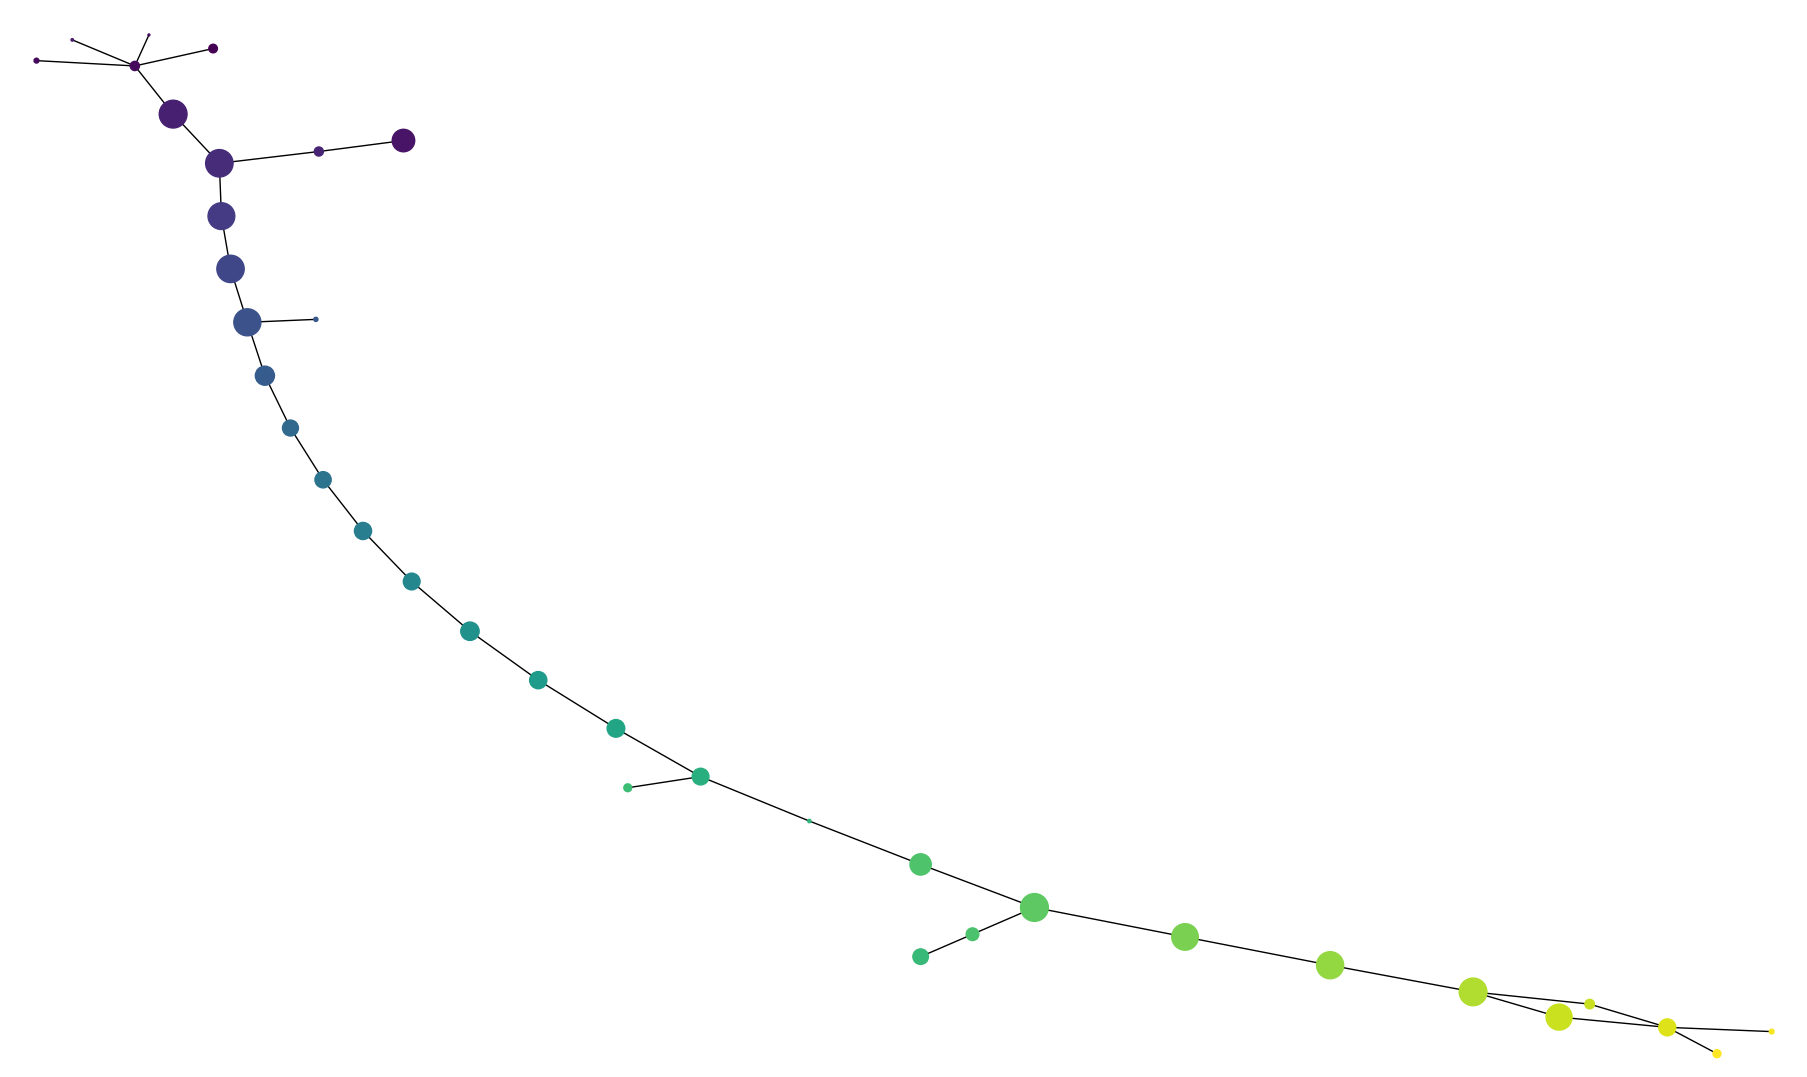
\includegraphics[width=0.4\textwidth]{images/benchmark/cat/benchmark_lmapper}
\end{figure}

On this second dataset lmapper is approximately 20\% faster than kmapper; again we see that lmapper's graph is again more robust to noise. There's only one connected component, and the main topological feature (the ring) is still captured.

\subsection{filterutils}
For an Eccentricity filter calculated with exponent set to $10$ and whith an euclidean distance, the filterutils package manage to get the following speedup (for reproducibility, run the file lmapper/test/test\_filterutils.py)

\begin{center}
	
	\begin{tabular}{ cc } 
		
		Threads & Speedup \\ 
		\hline
		1& 1\\ 
		2 & 1.83 \\ 
	\end{tabular}\\
	\bigskip
	Accuracy
\end{center}

To see the results, execute the test\_filterutils.py file in the lmapper test folder. On our machine we were limited to only 1 and 2 threads, but it would be interesting to test the scalability of the package on a machine capable of running more threads in parallel.
\subsection{predmap}
With predmap we managed to obtain the same results of Francesco Palma's master thesis (see the test folder of the package)
Here a table confronting the results. The small differences in the synthetic datasets are due to the fact that the dataset is not exactly the same used in Palma's work, since it has been regenerated through a random process and thus it is slightly different. The difference in the Wisconsin dataset however means that there's some slight difference in the algorithms. 

\begin{center}
	
	\begin{tabular}{ ccc } 
	
		&Palma's results & predmap (majority vote) \\ 
		\hline
		Synthetic dataset & 71.01\% & 70.85\% \\ 
		Wisconsin breast cancer dataset & 79.10\% & 79.78\% \\ 
	\end{tabular}\\
\bigskip
	Accuracy
\end{center}

\paragraph{Conclusions}
To conclude, the pure Python implementation of lmapper obtained a speedup of 10\% and 20\% compared to Kepler Mapper on the synthetic dataset of Palma and the Cat dataset of \cite{pythonmapper}. filterutils shows good speedup in calculating the eccentricity filter. Thanks to the implementation of the cutoff in the cutoff.py module the output is more robust to noise. predmap was capable of reproducing very closely the results of Francesco Palma's master thesis.

\pagebreak

\iffalse
\clearpage
\appendix
\fi

\bibliography{references.bib} 

\nocite{*}

\pagebreak



\end{document}
